%!TEX TS-program = xelatex
\documentclass[a4paper,14pt]{article}


%%% Работа с русским языком
\usepackage[english,russian]{babel}   %% загружает пакет многоязыковой вёрстки
\usepackage{fontspec}      %% подготавливает загрузку шрифтов Open Type, True Type и др.
\defaultfontfeatures{Ligatures={TeX},Renderer=Basic}  %% свойства шрифтов по умолчанию
\setmainfont[Ligatures={TeX,Historic}]{Times New Roman} %% задаёт основной шрифт документа
\setsansfont{Comic Sans MS}                    %% задаёт шрифт без засечек
\setmonofont{Courier New}
\usepackage{indentfirst}
\frenchspacing

\renewcommand{\epsilon}{\ensuremath{\varepsilon}}
\renewcommand{\phi}{\ensuremath{\varphi}}
\renewcommand{\kappa}{\ensuremath{\varkappa}}
\renewcommand{\le}{\ensuremath{\leqslant}}
\renewcommand{\leq}{\ensuremath{\leqslant}}
\renewcommand{\ge}{\ensuremath{\geqslant}}
\renewcommand{\geq}{\ensuremath{\geqslant}}
\renewcommand{\emptyset}{\varnothing}

%%% Дополнительная работа с математикой
\usepackage{amsmath,amsfonts,amssymb,amsthm,mathtools} % AMS
\usepackage{icomma} % "Умная" запятая: $0,2$ --- число, $0, 2$ --- перечисление

%% Номера формул
%\mathtoolsset{showonlyrefs=true} % Показывать номера только у тех формул, на которые есть \eqref{} в тексте.
%\usepackage{leqno} % Нумерация формул слева	

%% Перенос знаков в формулах (по Львовскому)
\newcommand*{\hm}[1]{#1\nobreak\discretionary{}
	{\hbox{$\mathsurround=0pt #1$}}{}}

%%% Работа с картинками
\usepackage{graphicx}  % Для вставки рисунков
\graphicspath{{images/}}  % папки с картинками
\setlength\fboxsep{3pt} % Отступ рамки \fbox{} от рисунка
\setlength\fboxrule{1pt} % Толщина линий рамки \fbox{}
\usepackage{wrapfig} % Обтекание рисунков текстом

%%% Работа с таблицами
\usepackage{array,tabularx,tabulary,booktabs} % Дополнительная работа с таблицами
\usepackage{longtable}  % Длинные таблицы
\usepackage{multirow} % Слияние строк в таблице
\usepackage{float}% http://ctan.org/pkg/float

%%% Программирование
\usepackage{etoolbox} % логические операторы


%%% Страница
\usepackage{extsizes} % Возможность сделать 14-й шрифт
\usepackage{geometry} % Простой способ задавать поля
\geometry{top=20mm}
\geometry{bottom=20mm}
\geometry{left=20mm}
\geometry{right=10mm}
%
%\usepackage{fancyhdr} % Колонтитулы
% 	\pagestyle{fancy}
%\renewcommand{\headrulewidth}{0pt}  % Толщина линейки, отчеркивающей верхний колонтитул
% 	\lfoot{Нижний левый}
% 	\rfoot{Нижний правый}
% 	\rhead{Верхний правый}
% 	\chead{Верхний в центре}
% 	\lhead{Верхний левый}
%	\cfoot{Нижний в центре} % По умолчанию здесь номер страницы

\usepackage{setspace} % Интерлиньяж
\onehalfspacing % Интерлиньяж 1.5
%\doublespacing % Интерлиньяж 2
%\singlespacing % Интерлиньяж 1

\usepackage{lastpage} % Узнать, сколько всего страниц в документе.

\usepackage{soul} % Модификаторы начертания

\usepackage{hyperref}
\usepackage[usenames,dvipsnames,svgnames,table,rgb]{xcolor}
\hypersetup{				% Гиперссылки
	unicode=true,           % русские буквы в раздела PDF
	pdftitle={Проектирование многоразрядного десятичного сумматора комбинационного типа},   % Заголовок
	pdfauthor={Подчезерцев Алексей},      % Автор
	pdfsubject={Проектирование многоразрядного десятичного сумматора комбинационного типа},      % Тема
	pdfcreator={Подчезерцев Алексей}, % Создатель
	pdfproducer={Подчезерцев Алексей}, % Производитель
	pdfkeywords={Теория автоматов} {МИЭМ} {ВШЭ}, % Ключевые слова
	colorlinks=true,       	% false: ссылки в рамках; true: цветные ссылки
	linkcolor=black,          % внутренние ссылки
	citecolor=black,        % на библиографию
	filecolor=magenta,      % на файлы
	urlcolor=black           % на URL
}
\makeatletter 
\def\@biblabel#1{#1. } 
\makeatother
\usepackage{cite} % Работа с библиографией
%\usepackage[superscript]{cite} % Ссылки в верхних индексах
%\usepackage[nocompress]{cite} % 
\usepackage{csquotes} % Еще инструменты для ссылок

\usepackage{multicol} % Несколько колонок

\usepackage{tikz} % Работа с графикой
\usepackage{pgfplots}
\usepackage{pgfplotstable}

% ГОСТ заголовки
\usepackage[font=small]{caption}
%\captionsetup[table]{justification=centering, labelsep = newline} % Таблицы по правобу краю
%\captionsetup[figure]{justification=centering} % Картинки по центру


\newcommand{\tablecaption}[1]{\addtocounter{table}{1}\small \begin{flushright}\tablename \ \thetable\end{flushright}%	
\begin{center}#1\end{center}}

\newcommand{\imref}[1]{рис.~\ref{#1}}

\usepackage{multirow}
\usepackage{spreadtab}
\newcolumntype{K}[1]{@{}>{\centering\arraybackslash}p{#1cm}@{}}


\usepackage{xparse}
\ExplSyntaxOn
\DeclareExpandableDocumentCommand{\juliandate}{ m m m }
{
	\juliandate_calc:nnnn { #1 } { #2 } { #3 } { \use:n }
}
\NewDocumentCommand{\storejuliandate}{ s m m m m }
{
	\IfBooleanTF{#1}
	{
		\juliandate_calc:nnnn { #3 } { #4 } { #5 } { \cs_set:Npx #2 }
	}
	{
		\juliandate_calc:nnnn { #3 } { #4 } { #5 } { \cs_new:Npx #2 }
	}
}
\cs_new:Npn \juliandate_calc:nnnn #1 #2 #3 #4 % #1 = day, #2 = month, #3 = year, #4 = what to do
{
	#4 
	{
		\int_eval:n
		{
			#1 +
			\int_div_truncate:nn { 153 * (#2 + 12 * \int_div_truncate:nn { 14 - #2 } { 12 } - 3) + 2 } { 5 } +
			365 * (#3 + 4800 - \int_div_truncate:nn { 14 - #2 } { 12 } ) +
			\int_div_truncate:nn { #3 + 4800 - \int_div_truncate:nn { 14 - #2 } { 12 } } { 4 } -
			\int_div_truncate:nn { #3 + 4800 - \int_div_truncate:nn { 14 - #2 } { 12 } } { 100 } + 
			\int_div_truncate:nn { #3 + 4800 - \int_div_truncate:nn { 14 - #2 } { 12 } } { 400 } -
			32045
		}
	}
}

\tl_new:N \l__juliandate_g_tl
\tl_new:N \l__juliandate_dg_tl
\tl_new:N \l__juliandate_c_tl
\tl_new:N \l__juliandate_dc_tl
\tl_new:N \l__juliandate_b_tl
\tl_new:N \l__juliandate_db_tl
\tl_new:N \l__juliandate_a_tl
\tl_new:N \l__juliandate_da_tl
\tl_new:N \l__juliandate_y_tl
\tl_new:N \l__juliandate_m_tl
\tl_new:N \l__juliandate_d_tl
\int_new:N \l_juliandate_day_int
\int_new:N \l_juliandate_month_int
\int_new:N \l_juliandate_year_int

\cs_new:Npn \__juliandate_set:nn #1 #2
{
	\tl_set:cx { l__juliandate_#1_tl } { \int_eval:n { #2 } }
}
\cs_new:Npn \__juliandate_use:n #1
{
	\tl_use:c { l__juliandate_#1_tl }
}
\cs_new_protected:Npn \juliandate_reverse:n #1
{
	\__juliandate_set:nn { g }
	{ \int_div_truncate:nn { #1 + 32044 } { 146097 } }
	\__juliandate_set:nn { dg }
	{ \int_mod:nn { #1 + 32044 } { 146097 } }
	\__juliandate_set:nn { c }
	{ \int_div_truncate:nn { ( \int_div_truncate:nn { \__juliandate_use:n { dg } } { 36524 } + 1) * 3 } { 4 } }
	\__juliandate_set:nn { dc }
	{ \__juliandate_use:n { dg } - \__juliandate_use:n { c } * 36524 }
	\__juliandate_set:nn { b }
	{ \int_div_truncate:nn { \__juliandate_use:n { dc } } { 1461 } }
	\__juliandate_set:nn { db }
	{ \int_mod:nn { \__juliandate_use:n { dc } } { 1461 } }
	\__juliandate_set:nn { a }
	{ \int_div_truncate:nn { ( \int_div_truncate:nn { \__juliandate_use:n { db } } { 365 } + 1) * 3 } { 4 } }
	\__juliandate_set:nn { da }
	{ \__juliandate_use:n { db } - \__juliandate_use:n { a } * 365 }
	\__juliandate_set:nn { y }
	{
		\__juliandate_use:n { g } * 400 + 
		\__juliandate_use:n { c } * 100 + 
		\__juliandate_use:n { b } * 4 + 
		\__juliandate_use:n { a }
	}
	\__juliandate_set:nn { m }
	{ \int_div_truncate:nn { \__juliandate_use:n { da } * 5 + 308 } { 153 } - 2 }
	\__juliandate_set:nn { d }
	{ \__juliandate_use:n { da } - \int_div_truncate:nn { (\__juliandate_use:n { m } + 4) * 153 } { 5 } + 122 }
	\int_set:Nn \l_juliandate_year_int
	{ \__juliandate_use:n { y } - 4800 + \int_div_truncate:nn { \__juliandate_use:n { m } + 2 } { 12 } }
	\int_set:Nn \l_juliandate_month_int
	{ \int_mod:nn { \__juliandate_use:n { m } + 2 } { 12 } + 1 }
	\int_set:Nn \l_juliandate_day_int
	{ \__juliandate_use:n { d } + 1 }
}
\cs_generate_variant:Nn \juliandate_reverse:n { x }

\NewDocumentCommand{\showday}{ m }
{
	\juliandate_reverse:n { #1 }
	\int_to_arabic:n { \l_juliandate_day_int }-
	\int_to_arabic:n { \l_juliandate_month_int }-
	\int_to_arabic:n { \l_juliandate_year_int }
}

\NewDocumentCommand{\tomorrow}{ }
{
	\group_begin:
	\juliandate_reverse:x { \juliandate_calc:nnnn { \day + 1 } { \month } { \year } { \use:n } }
	\day = \l_juliandate_day_int
	\month = \l_juliandate_month_int
	\year = \l_juliandate_year_int
	\today
	\group_end:
}
\NewDocumentCommand{\tomorrowof}{ m m m }
{
	\group_begin:
	\juliandate_reverse:x { \juliandate_calc:nnnn { #1 + 1 } { #2 } { #3 } { \use:n } }
	\day = \l_juliandate_day_int
	\month = \l_juliandate_month_int
	\year = \l_juliandate_year_int
	\today
	\group_end:
}
\ExplSyntaxOff

\RequirePackage{lscape}
\usepackage{pdflscape}




\usepackage[figure,table,page]{totalcount} 
\usepackage{lastpage} 
\makeatletter 
\long\def\@secondoffour#1#2#3#4{#2} 
\def\getlastpage{\ifx\r@LastPage\@undefined 0\else 
	\expandafter\@secondoffour\r@LastPage\@empty\@empty\fi} 
\makeatother 

\usepackage{array}
\newcolumntype{?}{!{\vrule width 2pt}}
\begin{document} % конец преамбулы, начало документа
\begin{titlepage}
	\begin{center}
		ФЕДЕРАЛЬНОЕ  ГОСУДАРСТВЕННОЕ АВТОНОМНОЕ \\
		ОБРАЗОВАТЕЛЬНОЕ УЧРЕЖДЕНИЕ ВЫСШЕГО ОБРАЗОВАНИЯ\\
		«НАЦИОНАЛЬНЫЙ ИССЛЕДОВАТЕЛЬСКИЙ УНИВЕРСИТЕТ\\
		«ВЫСШАЯ ШКОЛА ЭКОНОМИКИ»
	\end{center}
	
	\begin{center}
		\textbf{Московский институт электроники и математики}
		
		\textbf{Им. А.Н.Тихонова НИУ ВШЭ}
		
		\vspace{2ex}
		
		\textbf{Департамент компьютерной инженерии}
	\end{center}
	\vspace{1ex}	
	\begin{center}
		Подчезерцев Алексей Евгеньевич, группа БИВ172
		
	\end{center}	
	\vspace{1ex}
	\begin{center}
		\textbf{<<Проектирование многоразрядного десятичного сумматора
			комбинационного типа>>}
	\end{center}	
	\vspace{2ex}
	\begin{center}
		по дисциплине <<Теория автоматов>>

	\end{center}
	\vspace{2ex}
	\begin{flushright}
		Исполнитель:
		
		Студент группы БИВ172
		
		$\rule{5cm}{0.15mm}$ А.Е. Подчезерцев 
		
	\end{flushright}
	\vspace{3ex}
	\begin{flushright}
		Руководитель:
		
		$\rule{5cm}{0.15mm}$ И.И. Бирюков
	\end{flushright}
	\vfill
	\begin{center}
		Москва \the\year \, г.
	\end{center}
\end{titlepage}

\section{Исходные данные для проектирования}


\begin{enumerate}
	\item Количество десятичных разрядов: $3$;
	\item Двоично-десятичный код, в котором находятся числа: $8421+6$;
	\item Система логических элементов: ИЛИ-НЕ, И-НЕ;
	\item Критерий оптимальности элементов для проектирования логических схем: минимальное число логических элементов (ЛЭ) в проектируемых схемах;
	\item Тип триггера для проектирования схемы управления синхронный D-треггер;
	\item Временные параметры синхронизирующей серии импульсов логических элементов: 
	время задержки в любом ЛЭ: 1 нс; 
	импульсы синхронизации длительностью 2 нс со скважностью 1. 
\end{enumerate}

\section{Разработка алгоритма выполнения арифметических операций сложения и вычитания многоразрядных чисел в заданом двоично-десятичном коде}

\begin{table}[H]
	\begin{tabular}{|c|c|}
		\hline
		\multicolumn{1}{|l|}{Цифра} & \multicolumn{1}{l|}{код (8421+6)} \\ \hline
		0 & 0110 \\ \hline
		1 & 0111 \\ \hline
		2 & 1000 \\ \hline
		3 & 1001 \\ \hline
		4 & 1010 \\ \hline
		5 & 1011 \\ \hline
		6 & 1100 \\ \hline
		7 & 1101 \\ \hline
		8 & 1110 \\ \hline
		9 & 1111 \\ \hline
	\end{tabular}
\end{table}

\subsection{Разработка алгоритма для одноразрядных десятичных чисел, получение величины коррекции и критерии ее ввода}

\begin{table}[H]
	\centering
	\begin{tabular}{|c|c|c|c|c|c|c|c|c|c|c|}
		\hline
		     & 0110 & 0111 & 1000 & 1001 & 1010 & 1011 & 1100 & 1101 & 1110 & 1111 \\ \hline
		     & 0110 & 0111 & 1000 & 1001 & 1010 & 1011 & 1100 & 1101 & 1110 & 1111 \\
		0110 & 1100 & 1101 & 1110 & 1111 & 0000 & 0001 & 0010 & 0011 & 0100 & 0101 \\
		     & 1010 & 1010 & 1010 & 1010 & 1010 & 1010 & 1010 & 1010 & 1010 & 1010 \\ \hline
		     & 0111 & 1000 & 1001 & 1010 & 1011 & 1100 & 1101 & 1110 & 1111 & 0110 \\
		0111 & 1101 & 1110 & 1111 & 0000 & 0001 & 0010 & 0011 & 0100 & 0101 & 0110 \\
		     & 1010 & 1010 & 1010 & 1010 & 1010 & 1010 & 1010 & 1010 & 1010 &  -   \\ \hline
		     & 1000 & 1001 & 1010 & 1011 & 1100 & 1101 & 1110 & 1111 & 0110 & 0111 \\
		1000 & 1110 & 1111 & 0000 & 0001 & 0010 & 0011 & 0100 & 0101 & 0110 & 0111 \\
		     & 1010 & 1010 & 1010 & 1010 & 1010 & 1010 & 1010 & 1010 &  -   &  -   \\ \hline
		     & 1001 & 1010 & 1011 & 1100 & 1101 & 1110 & 1111 & 0110 & 0111 & 1000 \\
		1001 & 1111 & 0000 & 0001 & 0010 & 0011 & 0100 & 0101 & 0110 & 0111 & 1000 \\
		     & 1010 & 1010 & 1010 & 1010 & 1010 & 1010 & 1010 &  -   &  -   &  -   \\ \hline
		     & 1010 & 1011 & 1100 & 1101 & 1110 & 1111 & 0110 & 0111 & 1000 & 1001 \\
		1010 & 0000 & 0001 & 0010 & 0011 & 0100 & 0101 & 0110 & 0111 & 1000 & 1001 \\
		     & 1010 & 1010 & 1010 & 1010 & 1010 & 1010 &  -   &  -   &  -   &  -   \\ \hline
		     & 1011 & 1100 & 1101 & 1110 & 1111 & 0110 & 0111 & 1000 & 1001 & 1010 \\
		1011 & 0001 & 0010 & 0011 & 0100 & 0101 & 0110 & 0111 & 1000 & 1001 & 1010 \\
		     & 1010 & 1010 & 1010 & 1010 & 1010 &      &  -   &  -   &  -   &  -   \\ \hline
		     & 1100 & 1101 & 1110 & 1111 & 0110 & 0111 & 1000 & 1001 & 1010 & 1011 \\
		1100 & 0010 & 0011 & 0100 & 0101 & 0110 & 0111 & 1000 & 1001 & 1010 & 1011 \\
		     & 1010 & 1010 & 1010 & 1010 &  -   &  -   &  -   &  -   &  -   &  -   \\ \hline
		     & 1101 & 1110 & 1111 & 0110 & 0111 & 1000 & 1001 & 1010 & 1011 & 1100 \\
		1101 & 0011 & 0100 & 0101 & 0110 & 0111 & 1000 & 1001 & 1010 & 1011 & 1100 \\
		     & 1010 & 1010 & 1010 &  -   &  -   &  -   &  -   &  -   &  -   &  -   \\ \hline
		     & 1110 & 1111 & 0110 & 0111 & 1000 & 1001 & 1010 & 1011 & 1100 & 1101 \\
		1110 & 0100 & 0101 & 0110 & 0111 & 1000 & 1001 & 1010 & 1011 & 1100 & 1101 \\
		     & 1010 & 1010 &  -   &  -   &  -   &  -   &  -   &  -   &  -   &  -   \\ \hline
		     & 1111 & 0110 & 0111 & 1000 & 1001 & 1010 & 1011 & 1100 & 1101 & 1110 \\
		1111 & 0101 & 0110 & 0111 & 1000 & 1001 & 1010 & 1011 & 1100 & 1101 & 1110 \\
		     & 1010 &  -   &  -   &  -   &  -   &  -   &  -   &  -   &  -   &  -   \\ \hline
	\end{tabular}
\end{table}
Критерии ввода корректировки:

\begin{itemize}
	\item Если отсутствует единица переноса или получена недопустимая комбинация, корректировка вводится, единица переноса не вводится;
	\item Если присутствует единица переноса и получена допустимая комбинация, то вводится  корректировка $1010$, при этом единица переноса сохраняется;
\end{itemize}

\subsection{Обобщение полученного алгоритма на многоразрядные числа при выполнении операции сложения и вычитания}

\subsection{Приведение шести примеров на следующие случаи сложения}

\subsubsection{(+A)+(+B)=(+C)}

\begin{figure}[H]
	\centering
	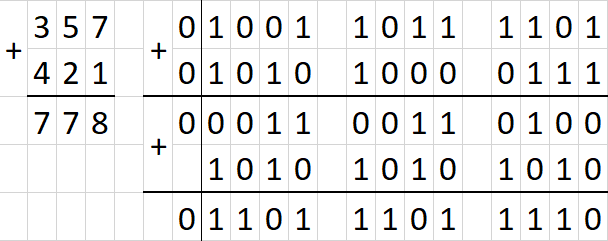
\includegraphics[width=0.7\linewidth]{images/ex1}
	\caption{}
	\label{fig:ex1}
\end{figure}



\subsubsection{(+A)+(-B)=(+C)}

\begin{figure}[H]
	\centering
	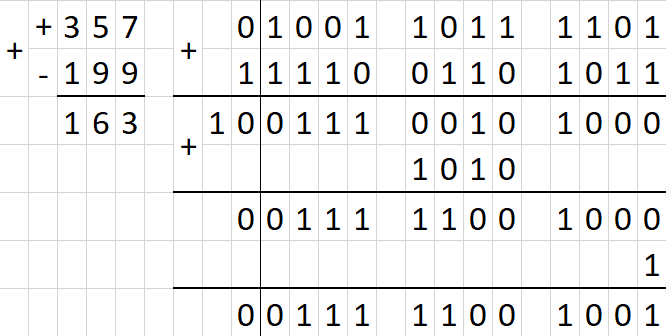
\includegraphics[width=0.7\linewidth]{images/ex2}
	\caption{}
	\label{fig:ex2}
\end{figure}



\subsubsection{(+A)+(-B)=(-C)}

\begin{figure}[H]
	\centering
	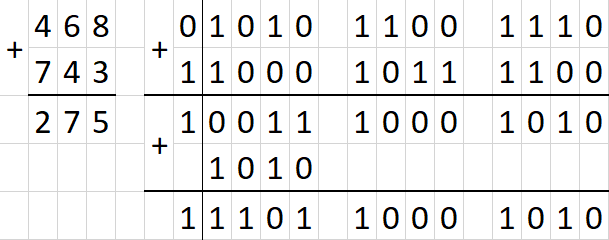
\includegraphics[width=0.7\linewidth]{images/ex3}
	\caption{}
	\label{fig:ex3}
\end{figure}



\subsubsection{(-A)+(-B)=(-C)}

\begin{figure}[H]
	\centering
	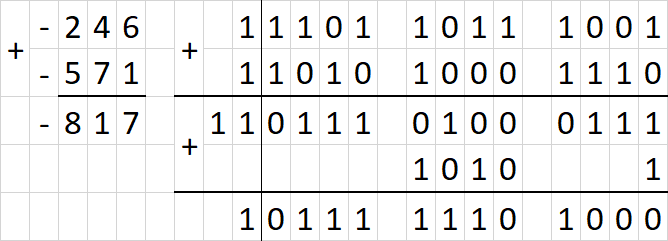
\includegraphics[width=0.7\linewidth]{images/ex4}
	\caption{}
	\label{fig:ex4}
\end{figure}



\subsubsection{(+A)+(+B)=(-C) — Переполнение разрядной сетки}

\begin{figure}[H]
	\centering
	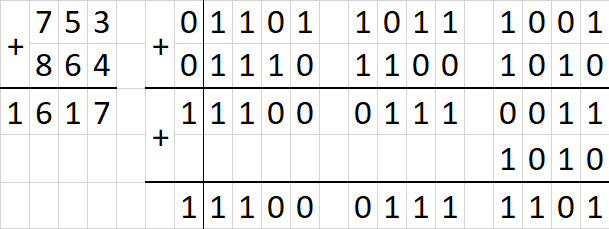
\includegraphics[width=0.7\linewidth]{images/ex5}
	\caption{}
	\label{fig:ex5}
\end{figure}




\subsubsection{(-A)+(-B)=(+C) — Переполнение разрядной сетки}

\begin{figure}[H]
	\centering
	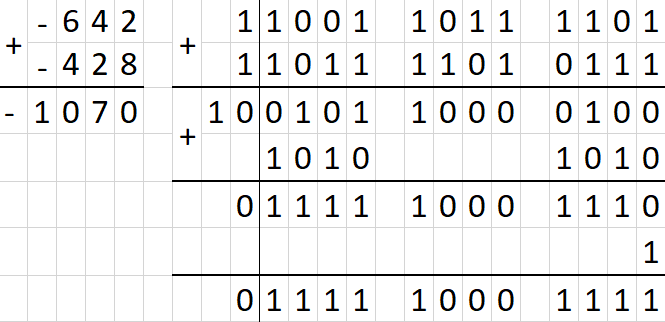
\includegraphics[width=0.7\linewidth]{images/ex6}
	\caption{}
	\label{fig:ex6}
\end{figure}

\section{Разработки функциональной схемы одноразрядного десятичного сумматора комбинационного типа}

\subsection{Разработка оптимальной схемы (с точки зрения критерия оптимальности) одноразрядного двоичного сумматора с учетом заданного базиса логических элементов}

Разработаем схему одноразрядного двоичного сумматора в базисе И-НЕ, ИЛИ-НЕ.

\begin{figure}[H]
	\centering
	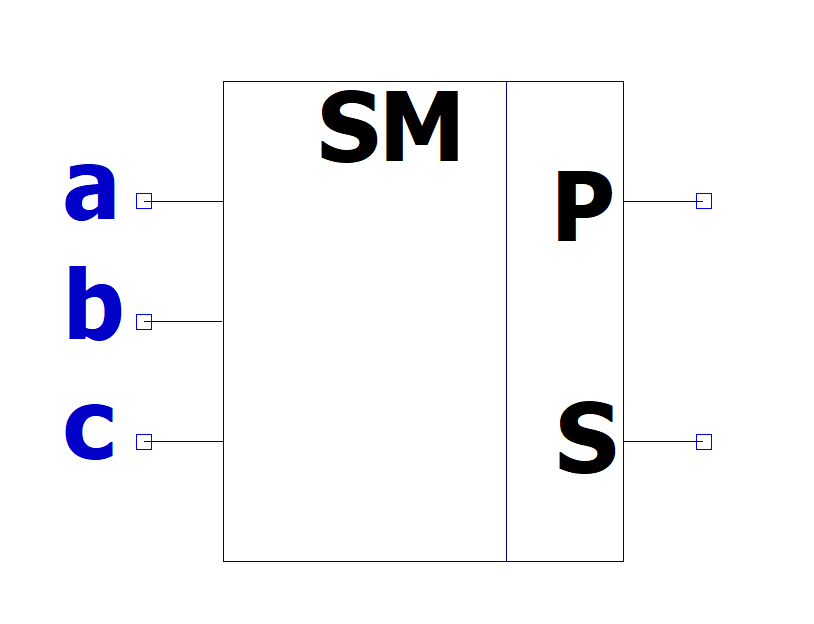
\includegraphics[width=0.3\linewidth]{schemas/sm_el}
	\caption{Одноразрядный двоичный сумматор}
	\label{fig:sm_el}
\end{figure}

Входы a, b - первое и второе слагаемое, c - перенос из младшего разряда, S - сумма, P - перенос в старший разряд (Рис. \ref{fig:sm}).
Далее будем изображать сумматор как на рис. \ref{fig:sm}.

\begin{table}[H]
	\begin{center}
		\caption{\label{tab:tab1} Таблица истинности для выходов S и P}
		\begin{tabular}{|c c c|c c|}
			\hline
			$a$ & $b$ & $c$ & $S$ & $P$ \\ \hline
			0 & 0 & 0 & 0 & 0 \\ 
			0 & 0 & 1 & 1 & 0 \\ 
			0 & 1 & 0 & 1 & 0 \\ 
			0 & 1 & 1 & 0 & 1 \\ 
			1 & 0 & 0 & 1 & 0 \\ 
			1 & 0 & 1 & 0 & 1 \\ 
			1 & 1 & 0 & 0 & 1 \\ 
			1 & 1 & 1 & 1 & 1 \\ \hline
		\end{tabular}
	\end{center}
\end{table}

\begin{table}[H]
	\begin{center}
		\caption{\label{tab:tab2} Диаграмма Вейча для функции $S$}
		\begin{tabular}{ccccc}
			& \multicolumn{2}{c}{$a$}                           & \multicolumn{2}{c}{$\overline{a}$}                          \\ \cline{2-5} 
			\multicolumn{1}{c|}{$b$}  & \multicolumn{1}{c|}{}  & \multicolumn{1}{c|}{1} & \multicolumn{1}{c|}{}  & \multicolumn{1}{c|}{1} \\ \cline{2-5} 
			\multicolumn{1}{c|}{$\overline{b}$} & \multicolumn{1}{c|}{1} & \multicolumn{1}{c|}{}  & \multicolumn{1}{c|}{1} & \multicolumn{1}{c|}{}  \\ \cline{2-5} 
			& $\overline{c}$                     & \multicolumn{2}{c}{$c$}                          & $\overline{c}$                     
		\end{tabular}
	\end{center}
\end{table}

\begin{table}[H]
	\begin{center}
		\caption{\label{tab:tab3} Диаграмма Вейча для функции $P$}
		\begin{tabular}{ccccc}
			& \multicolumn{2}{c}{$a$}                           & \multicolumn{2}{c}{$\overline{a}$}                          \\ \cline{2-5} 
			\multicolumn{1}{c|}{$b$}  & \multicolumn{1}{c|}{1}  & \multicolumn{1}{c|}{1} & \multicolumn{1}{c|}{1}  & \multicolumn{1}{c|}{} \\ \cline{2-5} 
			\multicolumn{1}{c|}{$\overline{b}$} & \multicolumn{1}{c|}{} & \multicolumn{1}{c|}{1}  & \multicolumn{1}{c|}{} & \multicolumn{1}{c|}{}  \\ \cline{2-5} 
			& $\overline{c}$                     & \multicolumn{2}{c}{$c$}                          & $\overline{c}$                     
		\end{tabular}
	\end{center}
\end{table}

\begin{table}[H]
	\begin{center}
		\caption{\label{tab:tab4} Диаграмма Вейча для функции $\overline{S}$}
		\begin{tabular}{ccccc}
			& \multicolumn{2}{c}{$a$}                           & \multicolumn{2}{c}{$\overline{a}$}                          \\ \cline{2-5} 
			\multicolumn{1}{c|}{$b$}  & \multicolumn{1}{c|}{1}  & \multicolumn{1}{c|}{} & \multicolumn{1}{c|}{1}  & \multicolumn{1}{c|}{} \\ \cline{2-5} 
			\multicolumn{1}{c|}{$\overline{b}$} & \multicolumn{1}{c|}{} & \multicolumn{1}{c|}{1}  & \multicolumn{1}{c|}{} & \multicolumn{1}{c|}{1}  \\ \cline{2-5} 
			& $\overline{c}$                     & \multicolumn{2}{c}{$c$}                          & $\overline{c}$                     
		\end{tabular}
	\end{center}
\end{table}

\begin{table}[H]
	\begin{center}
		\caption{\label{tab:tab5} Диаграмма Вейча для функции $\overline{P}$}
		\begin{tabular}{ccccc}
			& \multicolumn{2}{c}{$a$}                           & \multicolumn{2}{c}{$\overline{a}$}                          \\ \cline{2-5} 
			\multicolumn{1}{c|}{$b$}  & \multicolumn{1}{c|}{}  & \multicolumn{1}{c|}{} & \multicolumn{1}{c|}{}  & \multicolumn{1}{c|}{1} \\ \cline{2-5} 
			\multicolumn{1}{c|}{$\overline{b}$} & \multicolumn{1}{c|}{1} & \multicolumn{1}{c|}{}  & \multicolumn{1}{c|}{1} & \multicolumn{1}{c|}{1}  \\ \cline{2-5} 
			& $\overline{c}$                     & \multicolumn{2}{c}{$c$}                          & $\overline{c}$                     
		\end{tabular}
	\end{center}
\end{table}

\begin{equation*}
\begin{aligned}
	S &= abc + a\bar{b}\bar{c} + \bar{a}\bar{b}c + \bar{a}b\bar{c} = \overline{\overline{abc} * \overline{a\bar{b}\bar{c}} * \overline{\bar{a}\bar{b}c} * \overline{\bar{a}b\bar{c}}} - \text{8ЛЭ} \\
	S &= \overline{\overline{(\bar{a}+\bar{b}+c)} + \overline{(\bar{a}+b+\bar{c})} + \overline{(a+\bar{b}+\bar{c})} + \overline{(a+b+c)}} - \text{8ЛЭ}
\end{aligned}
\end{equation*}

\begin{equation*}
\begin{aligned}
	P &= ab + ac + bc = \overline{\overline{ab} * \overline{ac} * \overline{bc}} - \text{4ЛЭ} \\
	P &= \overline{\overline{(a+b)} + \overline{(a+c)} + \overline{(b+c)}} - \text{4ЛЭ}
\end{aligned}
\end{equation*}

\begin{equation*}
	S = \overline{(\bar{P} + abc) (a + b + c)} = \overline{\overline{(\bar{P} + \overline{\overline{abc}})} + \overline{(a+b+c)}} - \text{6ЛЭ}
\end{equation*}

Наиболее оптимальный вариант проектирования -- выразить S через P (экономия 2ЛЭ), P можно выразить любым удобным способом.
Потребуется 10 ЛЭ.

\begin{figure}[H]
	\centering
	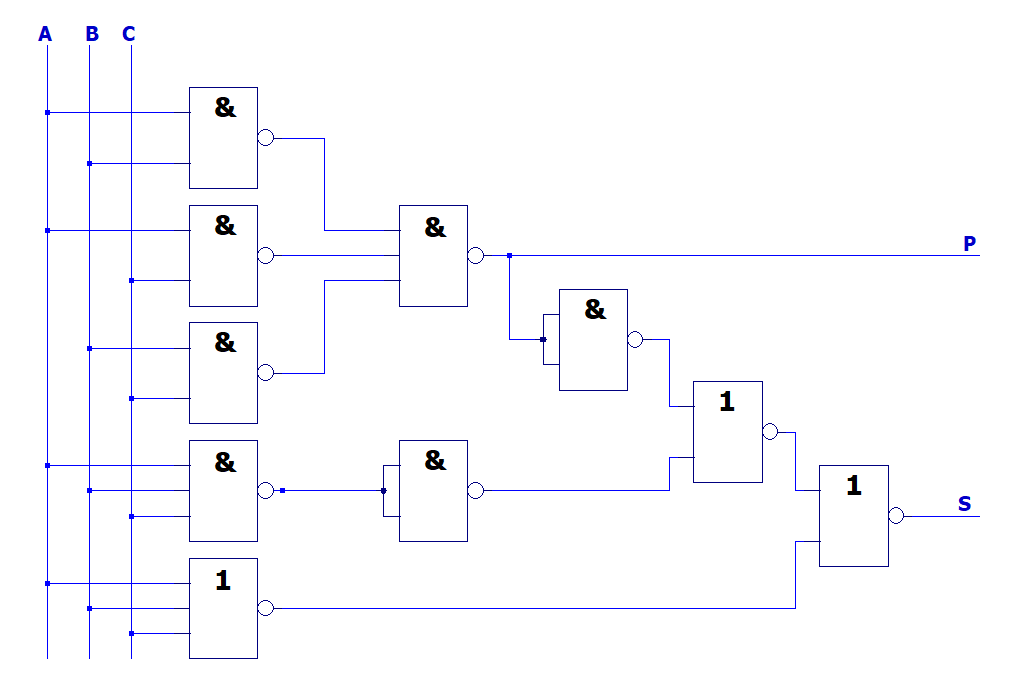
\includegraphics[width=\linewidth]{schemas/sm}
	\caption{Логическая схема одноразрядного двоичного сумматора}
	\label{fig:sm}
\end{figure}

\subsection{Разработка схемы коррекции}

Заметим, что при обработке сигнала в корректоре может быть или введена коррекция, или произведён перенос в следующий разряд.
Учтём это при проектировании.
$\gamma_8$, $\gamma_4$, $\gamma_2$, $\gamma_1$ -- результат сложения, П' -- перенос, получившийся при сложении.
К -- необходимость ввода коррекции, П -- признак переноса разряда.

\begin{table}[H]
	\centering
	\caption{\label{tab:dvKorr} Таблица истинности для функций $K$ и П в корректоре}
	\begin{tabular}{|c|c|c|c|c?c|c|}
		\hline
		$\gamma_8$ & $\gamma_4$ & $\gamma_2$ & $\gamma_1$ & П' & K & П \\ \hline
		0          & 0          & 0          & 0          & 0  & x & x \\ \hline
		0          & 0          & 0          & 0          & 1  & 1 & 0 \\ \hline
		0          & 0          & 0          & 1          & 0  & x & x \\ \hline
		0          & 0          & 0          & 1          & 1  & 1 & 0 \\ \hline
		0          & 0          & 1          & 0          & 0  & x & x \\ \hline
		0          & 0          & 1          & 0          & 1  & 1 & 0 \\ \hline
		0          & 0          & 1          & 1          & 0  & x & x \\ \hline
		0          & 0          & 1          & 1          & 1  & 1 & 0 \\ \hline
		0          & 1          & 0          & 0          & 0  & x & x \\ \hline
		0          & 1          & 0          & 0          & 1  & 1 & 0 \\ \hline
		0          & 1          & 0          & 1          & 0  & x & x \\ \hline
		0          & 1          & 0          & 1          & 1  & 1 & 0 \\ \hline
		0          & 1          & 1          & 0          & 0  & x & x \\ \hline
		0          & 1          & 1          & 0          & 1  & 0 & 1 \\ \hline
		0          & 1          & 1          & 1          & 0  & x & x \\ \hline
		0          & 1          & 1          & 1          & 1  & 0 & 1 \\ \hline
		1          & 0          & 0          & 0          & 0  & x & x \\ \hline
		1          & 0          & 0          & 0          & 1  & 0 & 1 \\ \hline
		1          & 0          & 0          & 1          & 0  & x & x \\ \hline
		1          & 0          & 0          & 1          & 1  & 0 & 1 \\ \hline
		1          & 0          & 1          & 0          & 0  & x & x \\ \hline
		1          & 0          & 1          & 0          & 1  & 0 & 1 \\ \hline
		1          & 0          & 1          & 1          & 0  & x & x \\ \hline
		1          & 0          & 1          & 1          & 1  & 0 & 1 \\ \hline
		1          & 1          & 0          & 0          & 0  & x & x \\ \hline
		1          & 1          & 0          & 0          & 1  & 0 & 1 \\ \hline
		1          & 1          & 0          & 1          & 0  & 1 & 0 \\ \hline
		1          & 1          & 0          & 1          & 1  & 0 & 1 \\ \hline
		1          & 1          & 1          & 0          & 0  & 1 & 0 \\ \hline
		1          & 1          & 1          & 0          & 1  & 0 & 1 \\ \hline
		1          & 1          & 1          & 1          & 0  & 1 & 0 \\ \hline
		1          & 1          & 1          & 1          & 1  & x & x \\ \hline
	\end{tabular}
\end{table}

\begin{table}[H]
	\begin{center}
		\caption{Коррекция}
		\begin{tabular}{cccccccccc}
			& \multicolumn{4}{c}{$\sqcap'$} & \multicolumn{4}{c}{$\bar{\sqcap'}$} &  \\
			& \multicolumn{2}{c}{$\gamma_8$} & \multicolumn{2}{c}{$\bar{\gamma_8}$} & \multicolumn{2}{c}{$\gamma_8$} & \multicolumn{2}{c}{$\bar{\gamma_8}$} &  \\ \cline{2-9}
			\multicolumn{1}{c|}{\multirow{2}{*}{$\gamma_4$}} & \multicolumn{1}{c|}{} & \multicolumn{1}{c|}{} & \multicolumn{1}{c|}{} & \multicolumn{1}{c|}{1} & \multicolumn{1}{c|}{x} & \multicolumn{1}{c|}{1} & \multicolumn{1}{c|}{x} & \multicolumn{1}{c|}{x} & $\bar{\gamma_1}$ \\ \cline{2-9}
			\multicolumn{1}{c|}{} & \multicolumn{1}{c|}{} & \multicolumn{1}{c|}{x} & \multicolumn{1}{c|}{} & \multicolumn{1}{c|}{1} & \multicolumn{1}{c|}{1} & \multicolumn{1}{c|}{1} & \multicolumn{1}{c|}{x} & \multicolumn{1}{c|}{x} & \multirow{2}{*}{$\gamma_1$} \\ \cline{2-9}
			\multicolumn{1}{c|}{\multirow{2}{*}{$\bar{\gamma_4}$}} & \multicolumn{1}{c|}{} & \multicolumn{1}{c|}{} & \multicolumn{1}{c|}{1} & \multicolumn{1}{c|}{1} & \multicolumn{1}{c|}{x} & \multicolumn{1}{c|}{x} & \multicolumn{1}{c|}{x} & \multicolumn{1}{c|}{x} &  \\ \cline{2-9}
			\multicolumn{1}{c|}{} & \multicolumn{1}{c|}{} & \multicolumn{1}{c|}{} & \multicolumn{1}{c|}{1} & \multicolumn{1}{c|}{1} & \multicolumn{1}{c|}{x} & \multicolumn{1}{c|}{x} & \multicolumn{1}{c|}{x} & \multicolumn{1}{c|}{x} & $\bar{\gamma_1}$ \\ \cline{2-9}
			\\
			& $\bar{\gamma_2}$ & \multicolumn{2}{c}{$\gamma_2$} & \multicolumn{2}{c}{$\bar{\gamma_2}$} & \multicolumn{2}{c}{$\gamma_2$} & $\bar{\gamma_2}$ & 
		\end{tabular}
	\end{center}
\end{table}

\begin{table}[H]
	\begin{center}
		\caption{Перенос}
		\begin{tabular}{cccccccccc}
			& \multicolumn{4}{c}{$\sqcap'$} & \multicolumn{4}{c}{$\bar{\sqcap'}$} &  \\
			& \multicolumn{2}{c}{$\gamma_8$} & \multicolumn{2}{c}{$\bar{\gamma_8}$} & \multicolumn{2}{c}{$\gamma_8$} & \multicolumn{2}{c}{$\bar{\gamma_8}$} &  \\ \cline{2-9}
			\multicolumn{1}{c|}{\multirow{2}{*}{$\gamma_4$}} & \multicolumn{1}{c|}{1} & \multicolumn{1}{c|}{1} & \multicolumn{1}{c|}{1} & \multicolumn{1}{c|}{} & \multicolumn{1}{c|}{x} & \multicolumn{1}{c|}{} & \multicolumn{1}{c|}{x} & \multicolumn{1}{c|}{x} & $\bar{\gamma_1}$ \\ \cline{2-9}
			\multicolumn{1}{c|}{} & \multicolumn{1}{c|}{1} & \multicolumn{1}{c|}{x} & \multicolumn{1}{c|}{1} & \multicolumn{1}{c|}{} & \multicolumn{1}{c|}{} & \multicolumn{1}{c|}{} & \multicolumn{1}{c|}{x} & \multicolumn{1}{c|}{x} & \multirow{2}{*}{$\gamma_1$} \\ \cline{2-9}
			\multicolumn{1}{c|}{\multirow{2}{*}{$\bar{\gamma_4}$}} & \multicolumn{1}{c|}{1} & \multicolumn{1}{c|}{1} & \multicolumn{1}{c|}{} & \multicolumn{1}{c|}{} & \multicolumn{1}{c|}{x} & \multicolumn{1}{c|}{x} & \multicolumn{1}{c|}{x} & \multicolumn{1}{c|}{x} &  \\ \cline{2-9}
			\multicolumn{1}{c|}{} & \multicolumn{1}{c|}{1} & \multicolumn{1}{c|}{1} & \multicolumn{1}{c|}{} & \multicolumn{1}{c|}{} & \multicolumn{1}{c|}{x} & \multicolumn{1}{c|}{x} & \multicolumn{1}{c|}{x} & \multicolumn{1}{c|}{x} & $\bar{\gamma_1}$ \\ \cline{2-9}
			\\
			& $\bar{\gamma_2}$ & \multicolumn{2}{c}{$\gamma_2$} & \multicolumn{2}{c}{$\bar{\gamma_2}$} & \multicolumn{2}{c}{$\gamma_2$} & $\bar{\gamma_2}$ & 
		\end{tabular}
	\end{center}
\end{table}


\begin{equation*}
\begin{aligned}
K &= \bar{\text{П'}} + \bar{\gamma_2}\bar{\gamma_8} + \bar{\gamma_8}\bar{\gamma_4} = \overline{\text{П'}*\overline{\bar{\gamma_2}\bar{\gamma_8}}*\overline{\bar{\gamma_8}\bar{\gamma_4}}}- \text{6ЛЭ} \\
K &= \overline{\overline{(\bar{\gamma_8}+\bar{\text{П'}})} + \overline{(\bar{\gamma_4}+\bar{\gamma_2}+\bar{\text{П'}})}} - \text{7ЛЭ}
\end{aligned}
\end{equation*}

\begin{equation*}
\begin{aligned}
\text{П} &= \gamma_8\text{П'} + \gamma_4\gamma_2\text{П'} = \overline{\overline{\gamma_8\text{П'}}*\overline{\gamma_4\gamma_2\text{П'}}} - \text{3ЛЭ} \\
\text{П} &= \overline{\bar{\text{П'}} + \overline{(\gamma_2+\gamma_8)} + \overline{(\gamma_8+\gamma_4)}} - \text{4ЛЭ}
\end{aligned}
\end{equation*}

Получим П с помощью 3ЛЭ, затем за 1ЛЭ получим из него К (Рис. \ref{fig:corr}).

\begin{figure}[H]
	\centering
	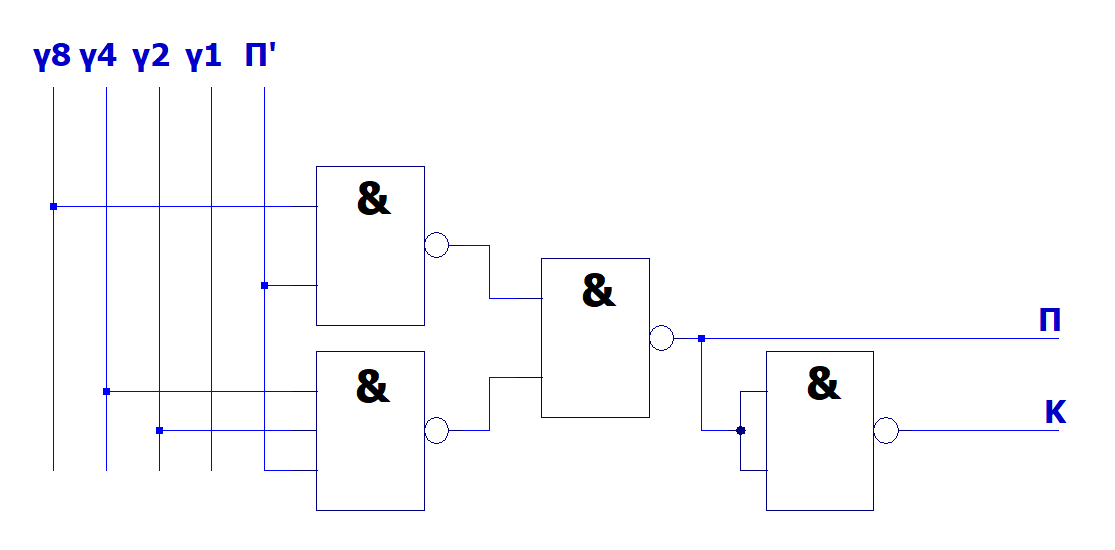
\includegraphics[width=\linewidth]{schemas/corr}
	\caption{Логическая схема корректора}
	\label{fig:corr}
\end{figure}

Получим П с помощью 3ЛЭ, затем за 1ЛЭ получим из него К (Рис. \ref{fig:corr}).

\begin{figure}[H]
	\centering
	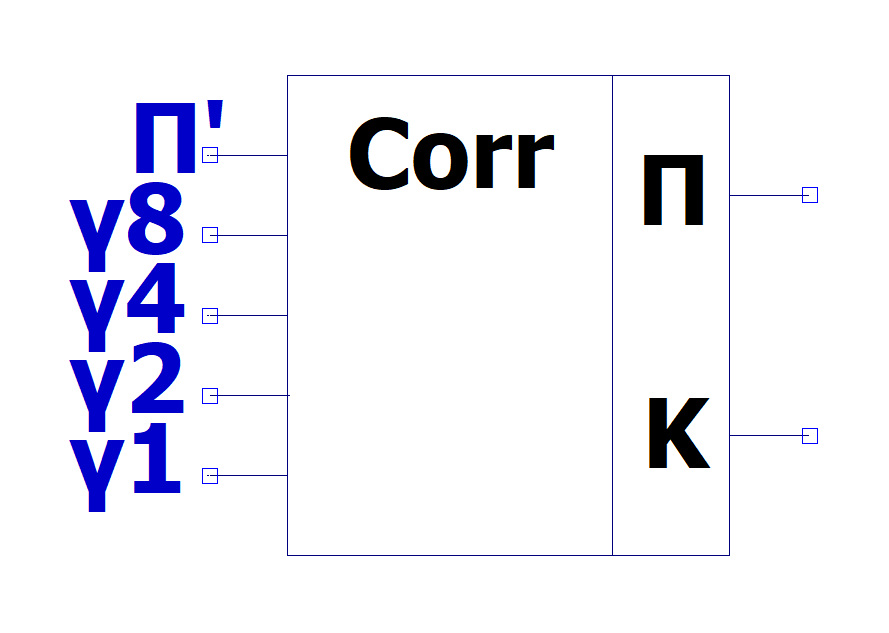
\includegraphics[width=0.3\linewidth]{schemas/corr_el}
	\caption{Обозначение схема корректора}
	\label{fig:corr_el}
\end{figure}

\subsection{Разработка схемы одноразрядного десятичного сумматора}

Итоговый вид:

\begin{figure}[H]
	\centering
	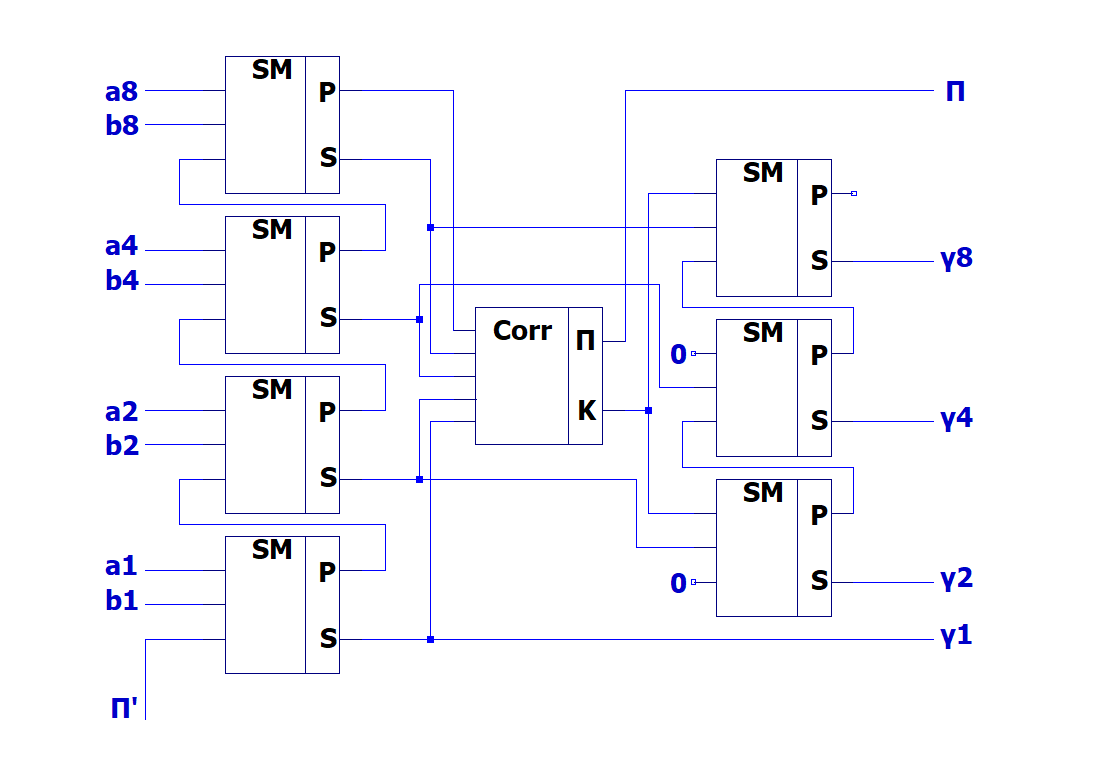
\includegraphics[width=\linewidth]{schemas/dc}
	\caption{Логическая схема одноразрядного сумматора}
	\label{fig:dc}
\end{figure}

Далее будем обозначать как:

\begin{figure}[H]
	\centering
	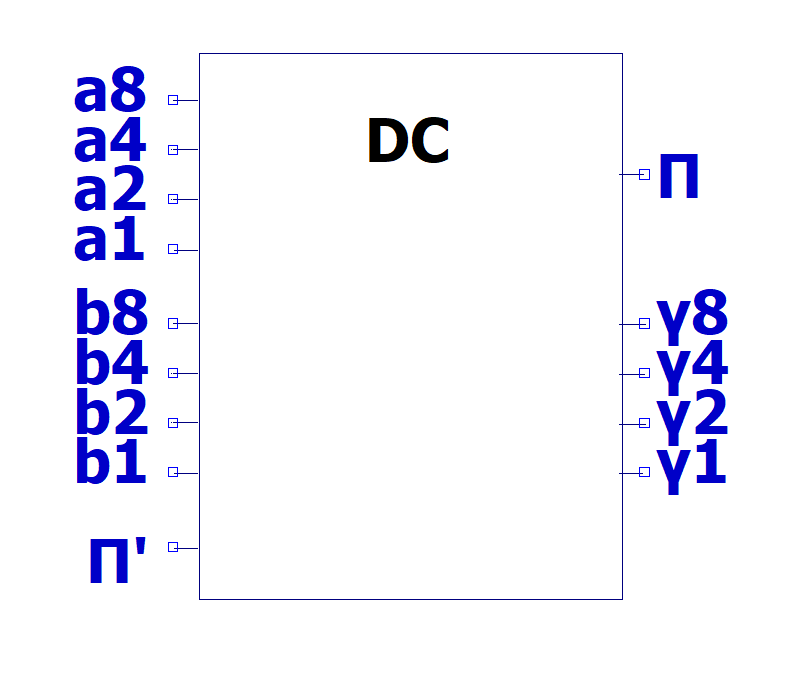
\includegraphics[width=0.3\linewidth]{schemas/dc_el}
	\caption{Одноразрядный сумматора}
	\label{fig:dcdc_el}
\end{figure}

\section{Разработка дополнительных схем для функционирования многоразрядного десятичного сумматора}

\subsection{Разработка преобразователя прямого кода в обратный для работы с отрицательными величинами}

Составим схему преобразователя в обратный код из прямого.
$a_i$ -- исходное значение, $\widehat{a_i}$ -- преобразованное. 
$a_0$ -- знак, не изменяется.

\begin{table}[H]
	\centering
	\caption{\label{tab:dvNeg} Таблица истинности для функций$\widehat{a_8}$, $\widehat{a_4}$, $\widehat{a_2}$, $\widehat{a_1}$}
	\begin{tabular}{|c|c|c|c|c|c|c|c|c|}
		\hline
		$a_0$ & $a_8$ & $a_4$ & $a_2$ & $a_1$ & $\widehat{a_8}$ & $\widehat{a_4}$ & $\widehat{a_2}$ & $\widehat{a_1}$ \\ \hline
		0     & 0     & 0     & 0     & 0     & x               & x               & x               & x               \\ \hline
		0     & 0     & 0     & 0     & 1     & x               & x               & x               & x               \\ \hline
		0     & 0     & 0     & 1     & 0     & x               & x               & x               & x               \\ \hline
		0     & 0     & 0     & 1     & 1     & x               & x               & x               & x               \\ \hline
		0     & 0     & 1     & 0     & 0     & x               & x               & x               & x               \\ \hline
		0     & 0     & 1     & 0     & 1     & x               & x               & x               & x               \\ \hline
		0     & 0     & 1     & 1     & 0     & 0               & 1               & 1               & 0               \\ \hline
		0     & 0     & 1     & 1     & 1     & 0               & 1               & 1               & 1               \\ \hline
		0     & 1     & 0     & 0     & 0     & 1               & 0               & 0               & 0               \\ \hline
		0     & 1     & 0     & 0     & 1     & 1               & 0               & 0               & 1               \\ \hline
		0     & 1     & 0     & 1     & 0     & 1               & 0               & 1               & 0               \\ \hline
		0     & 1     & 0     & 1     & 1     & 1               & 0               & 1               & 1               \\ \hline
		0     & 1     & 1     & 0     & 0     & 1               & 1               & 0               & 0               \\ \hline
		0     & 1     & 1     & 0     & 1     & 1               & 1               & 0               & 1               \\ \hline
		0     & 1     & 1     & 1     & 0     & 1               & 1               & 1               & 0               \\ \hline
		0     & 1     & 1     & 1     & 1     & 1               & 1               & 1               & 1               \\ \hline
		1     & 0     & 0     & 0     & 0     & x               & x               & x               & x               \\ \hline
		1     & 0     & 0     & 0     & 1     & x               & x               & x               & x               \\ \hline
		1     & 0     & 0     & 1     & 0     & x               & x               & x               & x               \\ \hline
		1     & 0     & 0     & 1     & 1     & x               & x               & x               & x               \\ \hline
		1     & 0     & 1     & 0     & 0     & x               & x               & x               & x               \\ \hline
		1     & 0     & 1     & 0     & 1     & x               & x               & x               & x               \\ \hline
		1     & 0     & 1     & 1     & 0     & 1               & 1               & 1               & 1               \\ \hline
		1     & 0     & 1     & 1     & 1     & 1               & 1               & 1               & 0               \\ \hline
		1     & 1     & 0     & 0     & 0     & 1               & 1               & 0               & 1               \\ \hline
		1     & 1     & 0     & 0     & 1     & 1               & 1               & 0               & 0               \\ \hline
		1     & 1     & 0     & 1     & 0     & 1               & 0               & 1               & 1               \\ \hline
		1     & 1     & 0     & 1     & 1     & 1               & 0               & 1               & 0               \\ \hline
		1     & 1     & 1     & 0     & 0     & 1               & 0               & 0               & 1               \\ \hline
		1     & 1     & 1     & 0     & 1     & 1               & 0               & 0               & 0               \\ \hline
		1     & 1     & 1     & 1     & 0     & 0               & 1               & 1               & 1               \\ \hline
		1     & 1     & 1     & 1     & 1     & 0               & 1               & 1               & 0               \\ \hline
	\end{tabular}
\end{table}

\begin{table}[H]
	\begin{minipage}{.5\linewidth}
		\caption{Диаграмма Вейча для функции $\hat{A_8}$}
		\centering
		\begin{tabular}{cccccccccc}
			& \multicolumn{4}{c}{$A_1$}                                                                           & \multicolumn{4}{c}{$\bar{A_1}$}                                                                    &                      \\
			& \multicolumn{2}{c}{$A_0$}                         & \multicolumn{2}{c}{$\bar{A_0}$}                   & \multicolumn{2}{c}{$A_0$}                         & \multicolumn{2}{c}{$\bar{A_0}$}                   &                      \\ \cline{2-9}
			\multicolumn{1}{c|}{\multirow{2}{*}{$A_8$}}       & \multicolumn{1}{c|}{1} & \multicolumn{1}{c|}{1} & \multicolumn{1}{c|}{1} & \multicolumn{1}{c|}{1} & \multicolumn{1}{c|}{1} & \multicolumn{1}{c|}{1} & \multicolumn{1}{c|}{1} & \multicolumn{1}{c|}{1} & $\bar{A_2}$            \\ \cline{2-9}
			\multicolumn{1}{c|}{}                           & \multicolumn{1}{c|}{1} & \multicolumn{1}{c|}{}  & \multicolumn{1}{c|}{1} & \multicolumn{1}{c|}{1} & \multicolumn{1}{c|}{1} & \multicolumn{1}{c|}{}  & \multicolumn{1}{c|}{1} & \multicolumn{1}{c|}{1} & \multirow{2}{*}{$A_2$} \\ \cline{2-9}
			\multicolumn{1}{c|}{\multirow{2}{*}{$\bar{A_8}$}} & \multicolumn{1}{c|}{x} & \multicolumn{1}{c|}{1} & \multicolumn{1}{c|}{}  & \multicolumn{1}{c|}{x} & \multicolumn{1}{c|}{x} & \multicolumn{1}{c|}{1} & \multicolumn{1}{c|}{}  & \multicolumn{1}{c|}{x} &                      \\ \cline{2-9}
			\multicolumn{1}{c|}{}                           & \multicolumn{1}{c|}{x} & \multicolumn{1}{c|}{x} & \multicolumn{1}{c|}{x} & \multicolumn{1}{c|}{x} & \multicolumn{1}{c|}{x} & \multicolumn{1}{c|}{x} & \multicolumn{1}{c|}{x} & \multicolumn{1}{c|}{x} & $\bar{A_2}$            \\ \cline{2-9}
			\\
			& $\bar{A_4}$              & \multicolumn{2}{c}{$A_4$}                         & \multicolumn{2}{c}{$\bar{A_4}$}                   & \multicolumn{2}{c}{$A_4$}                         & $\bar{A_4}$              &                     
		\end{tabular}
	\end{minipage}%
	\begin{minipage}{.5\linewidth}
		\centering
		\caption{Диаграмма Вейча для функции $\bar{\hat{A_8}}$}
\begin{tabular}{cccccccccc}
	& \multicolumn{4}{c}{$A_1$}                                                                         & \multicolumn{4}{c}{$\bar{A_1}$}                                                                   &                        \\
	& \multicolumn{2}{c}{$A_0$}                       & \multicolumn{2}{c}{$\bar{A_0}$}                 & \multicolumn{2}{c}{$A_0$}                       & \multicolumn{2}{c}{$\bar{A_0}$}                 &                        \\ \cline{2-9}
	\multicolumn{1}{c|}{\multirow{2}{*}{$A_8$}}       & \multicolumn{1}{c|}{}  & \multicolumn{1}{c|}{}  & \multicolumn{1}{c|}{}  & \multicolumn{1}{c|}{}  & \multicolumn{1}{c|}{}  & \multicolumn{1}{c|}{}  & \multicolumn{1}{c|}{}  & \multicolumn{1}{c|}{}  & $\bar{A_2}$            \\ \cline{2-9}
	\multicolumn{1}{c|}{}                             & \multicolumn{1}{c|}{}  & \multicolumn{1}{c|}{1} & \multicolumn{1}{c|}{}  & \multicolumn{1}{c|}{}  & \multicolumn{1}{c|}{}  & \multicolumn{1}{c|}{1} & \multicolumn{1}{c|}{}  & \multicolumn{1}{c|}{}  & \multirow{2}{*}{$A_2$} \\ \cline{2-9}
	\multicolumn{1}{c|}{\multirow{2}{*}{$\bar{A_8}$}} & \multicolumn{1}{c|}{x} & \multicolumn{1}{c|}{}  & \multicolumn{1}{c|}{1} & \multicolumn{1}{c|}{x} & \multicolumn{1}{c|}{x} & \multicolumn{1}{c|}{}  & \multicolumn{1}{c|}{1} & \multicolumn{1}{c|}{x} &                        \\ \cline{2-9}
	\multicolumn{1}{c|}{}                             & \multicolumn{1}{c|}{x} & \multicolumn{1}{c|}{x} & \multicolumn{1}{c|}{x} & \multicolumn{1}{c|}{x} & \multicolumn{1}{c|}{x} & \multicolumn{1}{c|}{x} & \multicolumn{1}{c|}{x} & \multicolumn{1}{c|}{x} & $\bar{A_2}$            \\ \cline{2-9}
	\\
	& $\bar{A_4}$            & \multicolumn{2}{c}{$A_4$}                       & \multicolumn{2}{c}{$\bar{A_4}$}                 & \multicolumn{2}{c}{$A_4$}                       & $\bar{A_4}$            &                       
\end{tabular}
	\end{minipage} 
\end{table}


\begin{table}[H]
	\begin{minipage}{.5\linewidth}
		\caption{Диаграмма Вейча для функции $\hat{A_4}$}
		\centering
		\begin{tabular}{cccccccccc}
			& \multicolumn{4}{c}{$A_1$}                                                                         & \multicolumn{4}{c}{$\bar{A_1}$}                                                                   &                        \\
			& \multicolumn{2}{c}{$A_0$}                       & \multicolumn{2}{c}{$\bar{A_0}$}                 & \multicolumn{2}{c}{$A_0$}                       & \multicolumn{2}{c}{$\bar{A_0}$}                 &                        \\ \cline{2-9}
			\multicolumn{1}{c|}{\multirow{2}{*}{$A_8$}}       & \multicolumn{1}{c|}{1} & \multicolumn{1}{c|}{}  & \multicolumn{1}{c|}{1} & \multicolumn{1}{c|}{}  & \multicolumn{1}{c|}{1} & \multicolumn{1}{c|}{}  & \multicolumn{1}{c|}{1} & \multicolumn{1}{c|}{}  & $\bar{A_2}$            \\ \cline{2-9}
			\multicolumn{1}{c|}{}                             & \multicolumn{1}{c|}{}  & \multicolumn{1}{c|}{1} & \multicolumn{1}{c|}{1} & \multicolumn{1}{c|}{}  & \multicolumn{1}{c|}{}  & \multicolumn{1}{c|}{1} & \multicolumn{1}{c|}{1} & \multicolumn{1}{c|}{}  & \multirow{2}{*}{$A_2$} \\ \cline{2-9}
			\multicolumn{1}{c|}{\multirow{2}{*}{$\bar{A_8}$}} & \multicolumn{1}{c|}{x} & \multicolumn{1}{c|}{1} & \multicolumn{1}{c|}{1} & \multicolumn{1}{c|}{x} & \multicolumn{1}{c|}{x} & \multicolumn{1}{c|}{1} & \multicolumn{1}{c|}{1} & \multicolumn{1}{c|}{x} &                        \\ \cline{2-9}
			\multicolumn{1}{c|}{}                             & \multicolumn{1}{c|}{x} & \multicolumn{1}{c|}{x} & \multicolumn{1}{c|}{x} & \multicolumn{1}{c|}{x} & \multicolumn{1}{c|}{x} & \multicolumn{1}{c|}{x} & \multicolumn{1}{c|}{x} & \multicolumn{1}{c|}{x} & $\bar{A_2}$            \\ \cline{2-9}
			\\
			& $\bar{A_4}$            & \multicolumn{2}{c}{$A_4$}                       & \multicolumn{2}{c}{$\bar{A_4}$}                 & \multicolumn{2}{c}{$A_4$}                       & $\bar{A_4}$            &                       
		\end{tabular}
	\end{minipage}%
	\begin{minipage}{.5\linewidth}
		\centering
		\caption{Диаграмма Вейча для функции $\bar{\hat{A_4}}$}
		\begin{tabular}{cccccccccc}
			& \multicolumn{4}{c}{$A_1$}                                                                         & \multicolumn{4}{c}{$\bar{A_1}$}                                                                   &                        \\
			& \multicolumn{2}{c}{$A_0$}                       & \multicolumn{2}{c}{$\bar{A_0}$}                 & \multicolumn{2}{c}{$A_0$}                       & \multicolumn{2}{c}{$\bar{A_0}$}                 &                        \\ \cline{2-9}
			\multicolumn{1}{c|}{\multirow{2}{*}{$A_8$}}       & \multicolumn{1}{c|}{}  & \multicolumn{1}{c|}{1} & \multicolumn{1}{c|}{}  & \multicolumn{1}{c|}{1} & \multicolumn{1}{c|}{}  & \multicolumn{1}{c|}{1} & \multicolumn{1}{c|}{}  & \multicolumn{1}{c|}{1} & $\bar{A_2}$            \\ \cline{2-9}
			\multicolumn{1}{c|}{}                             & \multicolumn{1}{c|}{1} & \multicolumn{1}{c|}{}  & \multicolumn{1}{c|}{}  & \multicolumn{1}{c|}{1} & \multicolumn{1}{c|}{1} & \multicolumn{1}{c|}{}  & \multicolumn{1}{c|}{}  & \multicolumn{1}{c|}{1} & \multirow{2}{*}{$A_2$} \\ \cline{2-9}
			\multicolumn{1}{c|}{\multirow{2}{*}{$\bar{A_8}$}} & \multicolumn{1}{c|}{x} & \multicolumn{1}{c|}{}  & \multicolumn{1}{c|}{}  & \multicolumn{1}{c|}{x} & \multicolumn{1}{c|}{x} & \multicolumn{1}{c|}{}  & \multicolumn{1}{c|}{}  & \multicolumn{1}{c|}{x} &                        \\ \cline{2-9}
			\multicolumn{1}{c|}{}                             & \multicolumn{1}{c|}{x} & \multicolumn{1}{c|}{x} & \multicolumn{1}{c|}{x} & \multicolumn{1}{c|}{x} & \multicolumn{1}{c|}{x} & \multicolumn{1}{c|}{x} & \multicolumn{1}{c|}{x} & \multicolumn{1}{c|}{x} & $\bar{A_2}$            \\ \cline{2-9}
			\\
			& $\bar{A_4}$            & \multicolumn{2}{c}{$A_4$}                       & \multicolumn{2}{c}{$\bar{A_4}$}                 & \multicolumn{2}{c}{$A_4$}                       & $\bar{A_4}$            &                       
		\end{tabular}
	\end{minipage} 
\end{table}

\begin{table}[H]
	\begin{minipage}{.5\linewidth}
		\caption{Диаграмма Вейча для функции $\hat{A_2}$}
		\centering
		\begin{tabular}{cccccccccc}
			& \multicolumn{4}{c}{$A_1$}                                                                         & \multicolumn{4}{c}{$\bar{A_1}$}                                                                   &                        \\
			& \multicolumn{2}{c}{$A_0$}                       & \multicolumn{2}{c}{$\bar{A_0}$}                 & \multicolumn{2}{c}{$A_0$}                       & \multicolumn{2}{c}{$\bar{A_0}$}                 &                        \\ \cline{2-9}
			\multicolumn{1}{c|}{\multirow{2}{*}{$A_8$}}       & \multicolumn{1}{c|}{}  & \multicolumn{1}{c|}{}  & \multicolumn{1}{c|}{}  & \multicolumn{1}{c|}{}  & \multicolumn{1}{c|}{}  & \multicolumn{1}{c|}{}  & \multicolumn{1}{c|}{}  & \multicolumn{1}{c|}{}  & $\bar{A_2}$            \\ \cline{2-9}
			\multicolumn{1}{c|}{}                             & \multicolumn{1}{c|}{1} & \multicolumn{1}{c|}{1} & \multicolumn{1}{c|}{1} & \multicolumn{1}{c|}{1} & \multicolumn{1}{c|}{1} & \multicolumn{1}{c|}{1} & \multicolumn{1}{c|}{1} & \multicolumn{1}{c|}{1} & \multirow{2}{*}{$A_2$} \\ \cline{2-9}
			\multicolumn{1}{c|}{\multirow{2}{*}{$\bar{A_8}$}} & \multicolumn{1}{c|}{x} & \multicolumn{1}{c|}{1} & \multicolumn{1}{c|}{1} & \multicolumn{1}{c|}{x} & \multicolumn{1}{c|}{x} & \multicolumn{1}{c|}{1} & \multicolumn{1}{c|}{1} & \multicolumn{1}{c|}{x} &                        \\ \cline{2-9}
			\multicolumn{1}{c|}{}                             & \multicolumn{1}{c|}{x} & \multicolumn{1}{c|}{x} & \multicolumn{1}{c|}{x} & \multicolumn{1}{c|}{x} & \multicolumn{1}{c|}{x} & \multicolumn{1}{c|}{x} & \multicolumn{1}{c|}{x} & \multicolumn{1}{c|}{x} & $\bar{A_2}$            \\ \cline{2-9}
			\\
			& $\bar{A_4}$            & \multicolumn{2}{c}{$A_4$}                       & \multicolumn{2}{c}{$\bar{A_4}$}                 & \multicolumn{2}{c}{$A_4$}                       & $\bar{A_4}$            &                       
		\end{tabular}
	\end{minipage}%
	\begin{minipage}{.5\linewidth}
		\centering
		\caption{Диаграмма Вейча для функции $\bar{\hat{A_2}}$}
		\begin{tabular}{cccccccccc}
			& \multicolumn{4}{c}{$A_1$}                                                                         & \multicolumn{4}{c}{$\bar{A_1}$}                                                                   &                        \\
			& \multicolumn{2}{c}{$A_0$}                       & \multicolumn{2}{c}{$\bar{A_0}$}                 & \multicolumn{2}{c}{$A_0$}                       & \multicolumn{2}{c}{$\bar{A_0}$}                 &                        \\ \cline{2-9}
			\multicolumn{1}{c|}{\multirow{2}{*}{$A_8$}}       & \multicolumn{1}{c|}{1} & \multicolumn{1}{c|}{1} & \multicolumn{1}{c|}{1} & \multicolumn{1}{c|}{1} & \multicolumn{1}{c|}{1} & \multicolumn{1}{c|}{1} & \multicolumn{1}{c|}{1} & \multicolumn{1}{c|}{1} & $\bar{A_2}$            \\ \cline{2-9}
			\multicolumn{1}{c|}{}                             & \multicolumn{1}{c|}{}  & \multicolumn{1}{c|}{}  & \multicolumn{1}{c|}{}  & \multicolumn{1}{c|}{}  & \multicolumn{1}{c|}{}  & \multicolumn{1}{c|}{}  & \multicolumn{1}{c|}{}  & \multicolumn{1}{c|}{}  & \multirow{2}{*}{$A_2$} \\ \cline{2-9}
			\multicolumn{1}{c|}{\multirow{2}{*}{$\bar{A_8}$}} & \multicolumn{1}{c|}{x} & \multicolumn{1}{c|}{}  & \multicolumn{1}{c|}{}  & \multicolumn{1}{c|}{x} & \multicolumn{1}{c|}{x} & \multicolumn{1}{c|}{}  & \multicolumn{1}{c|}{}  & \multicolumn{1}{c|}{x} &                        \\ \cline{2-9}
			\multicolumn{1}{c|}{}                             & \multicolumn{1}{c|}{x} & \multicolumn{1}{c|}{x} & \multicolumn{1}{c|}{x} & \multicolumn{1}{c|}{x} & \multicolumn{1}{c|}{x} & \multicolumn{1}{c|}{x} & \multicolumn{1}{c|}{x} & \multicolumn{1}{c|}{x} & $\bar{A_2}$            \\ \cline{2-9}
			\\
			& $\bar{A_4}$            & \multicolumn{2}{c}{$A_4$}                       & \multicolumn{2}{c}{$\bar{A_4}$}                 & \multicolumn{2}{c}{$A_4$}                       & $\bar{A_4}$            &                       
		\end{tabular}
	\end{minipage} 
\end{table}

\begin{table}[H]
	\begin{minipage}{.5\linewidth}
		\caption{Диаграмма Вейча для функции $\hat{A_1}$}
		\centering
		\begin{tabular}{cccccccccc}
			& \multicolumn{4}{c}{$A_1$} & \multicolumn{4}{c}{$\bar{A_1}$} &  \\
			& \multicolumn{2}{c}{$A_0$} & \multicolumn{2}{c}{$\bar{A_0}$} & \multicolumn{2}{c}{$A_0$} & \multicolumn{2}{c}{$\bar{A_0}$} &  \\ \cline{2-9}
			\multicolumn{1}{c|}{\multirow{2}{*}{$A_8$}} & \multicolumn{1}{c|}{} & \multicolumn{1}{c|}{} & \multicolumn{1}{c|}{1} & \multicolumn{1}{c|}{1} & \multicolumn{1}{c|}{1} & \multicolumn{1}{c|}{1} & \multicolumn{1}{c|}{} & \multicolumn{1}{c|}{} & $\bar{A_2}$ \\ \cline{2-9}
			\multicolumn{1}{c|}{} & \multicolumn{1}{c|}{} & \multicolumn{1}{c|}{} & \multicolumn{1}{c|}{1} & \multicolumn{1}{c|}{1} & \multicolumn{1}{c|}{1} & \multicolumn{1}{c|}{1} & \multicolumn{1}{c|}{} & \multicolumn{1}{c|}{} & \multirow{2}{*}{$A_2$} \\ \cline{2-9}
			\multicolumn{1}{c|}{\multirow{2}{*}{$\bar{A_8}$}} & \multicolumn{1}{c|}{x} & \multicolumn{1}{c|}{} & \multicolumn{1}{c|}{1} & \multicolumn{1}{c|}{x} & \multicolumn{1}{c|}{x} & \multicolumn{1}{c|}{1} & \multicolumn{1}{c|}{} & \multicolumn{1}{c|}{x} &  \\ \cline{2-9}
			\multicolumn{1}{c|}{} & \multicolumn{1}{c|}{x} & \multicolumn{1}{c|}{x} & \multicolumn{1}{c|}{x} & \multicolumn{1}{c|}{x} & \multicolumn{1}{c|}{x} & \multicolumn{1}{c|}{x} & \multicolumn{1}{c|}{x} & \multicolumn{1}{c|}{x} & $\bar{A_2}$ \\ \cline{2-9}
			\\
			& $\bar{A_4}$ & \multicolumn{2}{c}{$A_4$} & \multicolumn{2}{c}{$\bar{A_4}$} & \multicolumn{2}{c}{$A_4$} & $\bar{A_4}$ & 
		\end{tabular}
	\end{minipage}%
	\begin{minipage}{.5\linewidth}
		\centering
		\caption{Диаграмма Вейча для функции $\bar{\hat{A_1}}$}
		\begin{tabular}{cccccccccc}
			& \multicolumn{4}{c}{$A_1$} & \multicolumn{4}{c}{$\bar{A_1}$} &  \\
			& \multicolumn{2}{c}{$A_0$} & \multicolumn{2}{c}{$\bar{A_0}$} & \multicolumn{2}{c}{$A_0$} & \multicolumn{2}{c}{$\bar{A_0}$} &  \\ \cline{2-9}
			\multicolumn{1}{c|}{\multirow{2}{*}{$A_8$}} & \multicolumn{1}{c|}{1} & \multicolumn{1}{c|}{1} & \multicolumn{1}{c|}{} & \multicolumn{1}{c|}{} & \multicolumn{1}{c|}{} & \multicolumn{1}{c|}{} & \multicolumn{1}{c|}{1} & \multicolumn{1}{c|}{1} & $\bar{A_2}$ \\ \cline{2-9}
			\multicolumn{1}{c|}{} & \multicolumn{1}{c|}{1} & \multicolumn{1}{c|}{1} & \multicolumn{1}{c|}{} & \multicolumn{1}{c|}{} & \multicolumn{1}{c|}{} & \multicolumn{1}{c|}{} & \multicolumn{1}{c|}{1} & \multicolumn{1}{c|}{1} & \multirow{2}{*}{$A_2$} \\ \cline{2-9}
			\multicolumn{1}{c|}{\multirow{2}{*}{$\bar{A_8}$}} & \multicolumn{1}{c|}{x} & \multicolumn{1}{c|}{1} & \multicolumn{1}{c|}{} & \multicolumn{1}{c|}{x} & \multicolumn{1}{c|}{x} & \multicolumn{1}{c|}{} & \multicolumn{1}{c|}{1} & \multicolumn{1}{c|}{x} &  \\ \cline{2-9}
			\multicolumn{1}{c|}{} & \multicolumn{1}{c|}{x} & \multicolumn{1}{c|}{x} & \multicolumn{1}{c|}{x} & \multicolumn{1}{c|}{x} & \multicolumn{1}{c|}{x} & \multicolumn{1}{c|}{x} & \multicolumn{1}{c|}{x} & \multicolumn{1}{c|}{x} & $\bar{A_2}$ \\ \cline{2-9}
			\\
			& $\bar{A_4}$ & \multicolumn{2}{c}{$A_4$} & \multicolumn{2}{c}{$\bar{A_4}$} & \multicolumn{2}{c}{$A_4$} & $\bar{A_4}$ & 
		\end{tabular}
	\end{minipage} 
\end{table}

\begin{equation*}
\begin{aligned}
\widehat{A_8} &= \bar{a_2} + \bar{a_4} + \bar{a_0}a_8 + a_0\bar{a_8} = \overline{a_2*a_4*\overline{\bar{a_0}a_8}*\overline{a_0\bar{a_8}}} - \text{5ЛЭ|3ЛЭ} \\
\widehat{A_8} &= \overline{abc+\bar{a_0}\bar{a_8}} = \overline{\overline{(\bar{a_0}+\bar{a_8}+\bar{a_4})}+\overline{(a_0+a_8)}} - \text{6ЛЭ|3ЛЭ}
\end{aligned}
\end{equation*}

\begin{equation*}
\begin{aligned}
\widehat{A_4} &= a_0\bar{a_4}\bar{a_2} + cd + \bar{a_0}a_4 = \overline{\overline{a_0\bar{a_4}\bar{a_2}}*\overline{cd}*\overline{\bar{a_0}a_4}} - \text{7ЛЭ|4ЛЭ} \\
\widehat{A_4} &= \overline{ac\bar{a_2} + \bar{a_0}\bar{a_4}}  = 
\overline{\overline{(a_0+\bar{a_4}+a_2)}+\overline{(a_0+a_4)}}- \text{4ЛЭ|3ЛЭ}
\end{aligned}
\end{equation*}

\begin{equation*}
\begin{aligned}
\widehat{A_2} &= a_2 - \text{0ЛЭ}
\end{aligned}
\end{equation*}

\begin{equation*}
\begin{aligned}
\widehat{A_1} &= \bar{a_0}a_1 + a_0\bar{a_1} = \overline{\overline{\bar{a_0}a_1}*a_0\bar{a_1}} - \text{5ЛЭ|3ЛЭ} \\
\widehat{A_1} &= \overline{ae+\bar{a_0}\bar{a_1}} = \overline{\overline{(\bar{a_0}+\bar{a_1})}+\overline{(a_0+a_1)}} - \text{5ЛЭ|3ЛЭ}
\end{aligned}
\end{equation*}

Через черту указано количество логических элементов без учёта отрицания простых сигналов.

Построим итоговую схему на основе данных:

\begin{figure}[H]
	\centering
	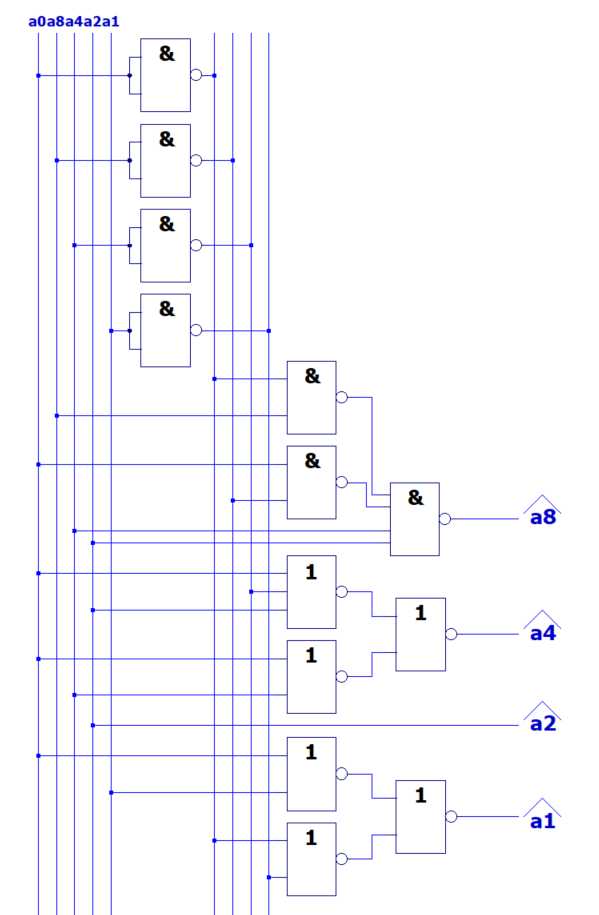
\includegraphics[width=0.9\linewidth]{schemas/pr}
	\caption{Логическая схема преобразователя}
	\label{fig:pr}
\end{figure}

Далее схему будем обозначать следующим образом:

\begin{figure}[H]
	\centering
	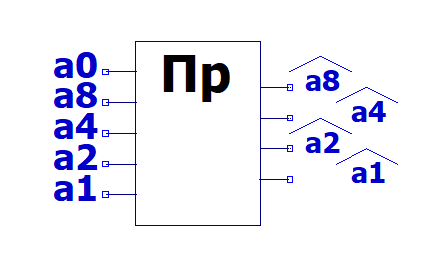
\includegraphics[width=0.3\linewidth]{schemas/pr_el}
	\caption{Обозначение схемы преобразователя}
	\label{fig:pr_el}
\end{figure}

\subsection{Разработка схемы, фиксирующей переполнение разрядной сетки}

Переполнение разрядной сетки происходит, когда:
\begin{itemize}
	\item При сложении двух положительных величин получается отрицательный результат.
	
	\item При сложении двух отрицательных величин получается положительный результат.	
\end{itemize}

\begin{table}[H]
	\begin{center}
		\caption{\label{tab:perSet} Таблица истинности для функции $\varphi$}
		
		\begin{tabular}{|l|l|l|l|}
			\hline
			a0 & b0 & c0 & $\varphi$ \\ \hline
			0  & 0  & 0  & 0  \\ \hline
			0  & 0  & 1  & 1  \\ \hline
			0  & 1  & 0  & 0  \\ \hline
			0  & 1  & 1  & 0  \\ \hline
			1  & 0  & 0  & 0  \\ \hline
			1  & 0  & 1  & 0  \\ \hline
			1  & 1  & 0  & 1  \\ \hline
			1  & 1  & 1  & 0  \\ \hline
		\end{tabular}
	\end{center}
\end{table}

\begin{table}[H]
	\begin{center}
		\caption{\label{tab:perSet_force} Диаграмма Вейча для функции  $\varphi$}
		
		\begin{tabular}{ccccc}
			& \multicolumn{2}{c}{$a_0$}                      & \multicolumn{2}{c}{$a_0$}                      \\ \cline{2-5} 
			\multicolumn{1}{c|}{$b_0$} & \multicolumn{1}{c|}{1} & \multicolumn{1}{c|}{} & \multicolumn{1}{c|}{}  & \multicolumn{1}{c|}{} \\ \cline{2-5} 
			\multicolumn{1}{c|}{$b_0$} & \multicolumn{1}{c|}{}  & \multicolumn{1}{c|}{} & \multicolumn{1}{c|}{1} & \multicolumn{1}{c|}{} \\ \cline{2-5} 
			& $\bar{c_0}$            & \multicolumn{2}{c}{$c_0$}                      & $\bar{c_0}$          
		\end{tabular}
	\end{center}
\end{table}

\begin{table}[H]
	\begin{center}
		\caption{\label{tab:perSet_ve} Диаграмма Вейча для функции  $\bar{\varphi}$}
		
		\begin{tabular}{ccccc}
			& \multicolumn{2}{c}{$a_0$}                           & \multicolumn{2}{c}{$\bar{a_0}$}                          \\ \cline{2-5} 
			\multicolumn{1}{c|}{$b_0$}  & \multicolumn{1}{c|}{}  & \multicolumn{1}{c|}{1} & \multicolumn{1}{c|}{1} & \multicolumn{1}{c|}{1} \\ \cline{2-5} 
			\multicolumn{1}{c|}{$\bar{b_0}$} & \multicolumn{1}{c|}{1} & \multicolumn{1}{c|}{1} & \multicolumn{1}{c|}{}  & \multicolumn{1}{c|}{1} \\ \cline{2-5} 
			& $\bar{c_0}$                    & \multicolumn{2}{c}{$c_0$}                           & $\bar{c_0}$                   
		\end{tabular}
	\end{center}
\end{table}

$$\varphi = ab\bar{c} + \bar{a}\bar{b}c =\overline{ \overline{ab\bar{c}} + \overline{\bar{a}\bar{b}c}} \text{ --  6ЛЭ}$$

$$\varphi = \overline{a\bar{b} + bc + \bar{a}\bar{c}} =  \overline{\overline{(\bar{a} + b)} +\overline{(\bar{b} + \bar{c})} + \overline{(a + c)}} \text{ --  7ЛЭ}$$

\begin{figure}[H]
	\centering
	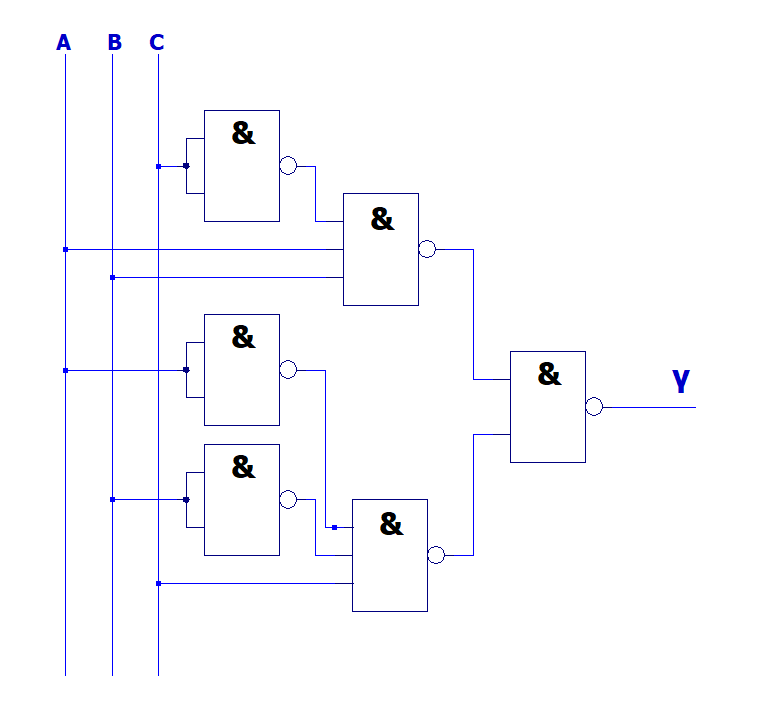
\includegraphics[width=0.5\linewidth]{schemas/per}
	\caption{Логическая схема, фиксирующая переполнение разрядной сетки}
	\label{fig:per}
\end{figure}

В дальнейшем будем обозначать эту схему следующим образом:

\begin{figure}[H]
	\centering
	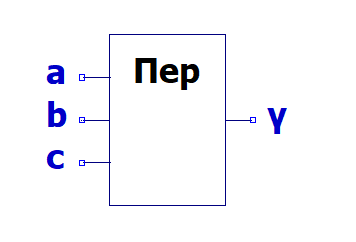
\includegraphics[width=0.2\linewidth]{schemas/per_el}
	\caption{Обозначение логической схемы, фиксирующей переполнение разрядной сетки}
	\label{fig:per_el}
\end{figure}

\subsection{Разработка схемы для определения знака суммы}

Правило сложения чисел в обратном коде гласит, что при выполнении операции знаковые разряды участвуют в сложении наравне с остальными разрядами. При этом учитывается  перенос в знаковый разряд и перенос из знакового разряда. Поэтому для получения знака результата можно использовать  одноразрядный двоичный сумматор.

\begin{figure}[H]
	\centering
	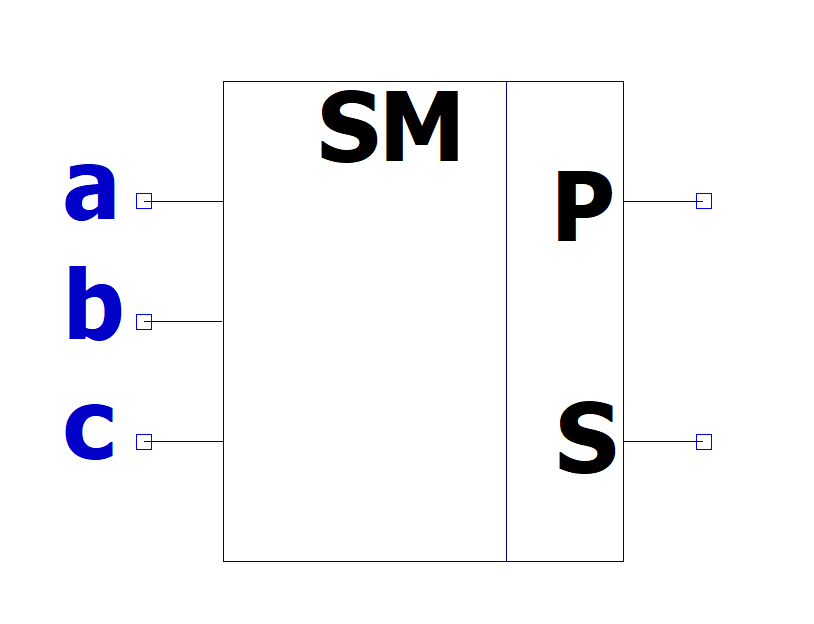
\includegraphics[width=0.3\linewidth]{schemas/sm_el}
	\caption{Одноразрядный двоичный сумматор}
	\label{fig:sm_el_2}
\end{figure}

\section{Разработки функциональной схемы многоразрядного десятичного сумматора}

Обозначим слагаемые на входе сумматора:

\begin{itemize}	
	\item A = a$_0$ a$_1$ a$_2$ a$_3$, где a$_0$ -- знак числа, a$_i$ -- десятичная цифра, которая представляется в двоично-десятичном коде следующим образом:
	a$_i = a^i_8 a^i_4 a^i_2 a^i_1$;
	
	\item B = b$_0$ b$_1$ b$_2$ b$_3$, где b$_0$ -- знак числа, b$_i = \beta^i_8 \beta^i_4 \beta^i_2 \beta^i_1$.	
\end{itemize}

Результат сложения обозначим:
\begin{itemize}	
	\item С = с$_0$ с$_1$ с$_2$ с$_3$, где с$_0$ -- знак числа, с$_i = \gamma^i_8 \gamma^i_4 \gamma^i_2 \gamma^i_1$.	
\end{itemize}

Используя все полученные результаты, можно построить структурную схему 3-разрядного десятичного сумматора.

\begin{figure}[H]
	\centering
	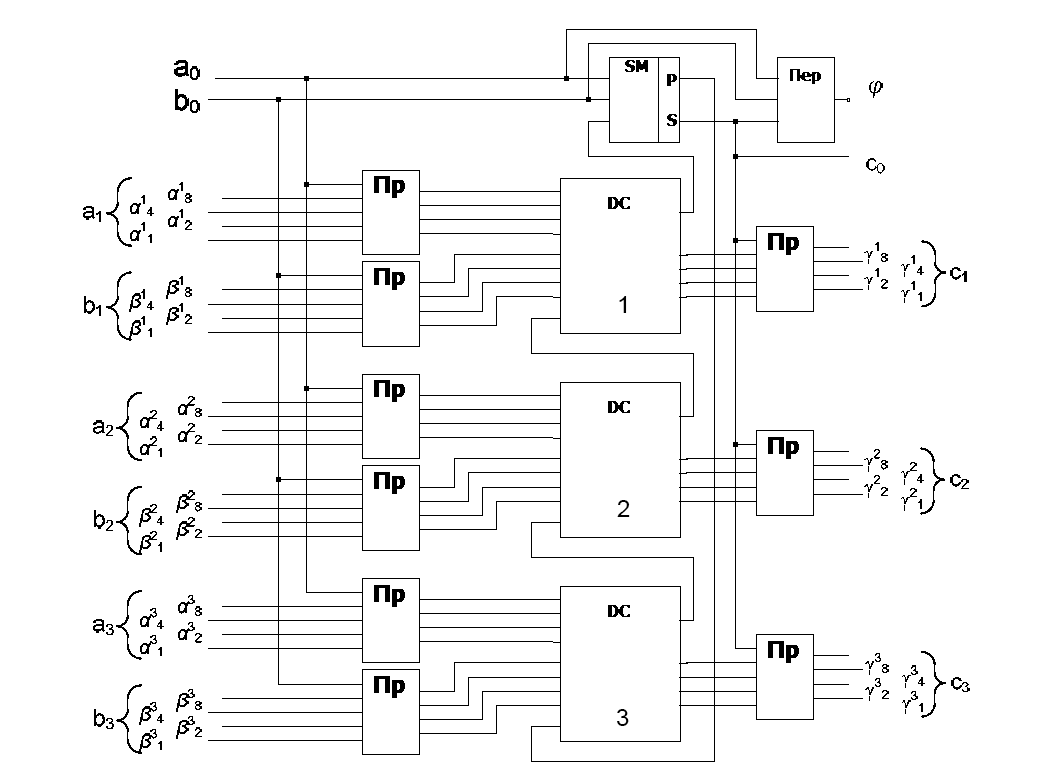
\includegraphics[width=\linewidth]{schemas/3Sum}
	\caption{Логическая схема 3-разрядного десятичного сумматора}
	\label{fig:3razrSum}
\end{figure}


\section{Разработка устройства управления для многоразрядного десятичного сумматора}

Для корректной работы устройства в системе должны присутствовать 4 синхроимпульса (СИ1, СИ2, СИ3, СИ4).

\begin{itemize}
	\item СИ1. Первый импульс позволяет записать 2 операнда во входные регистры, сразу после этого величины появляются на входах сумматора и сумматор начинает свою работу;
	
	\item СИ2. Второй импульс записывает в выходной регистр результат суммирования;
	
	\item СИ3. Третий импульс позволяет записать в регистр признаков все признаки результатов;
	
	\item СИ4. Останавливает процесс вычислений.
\end{itemize} 

\subsection{Разработка входных и выходных регистров хранения числовой информации, участвующей в операции сложения}

Регистры входа и выхода имеют одинаковую структуру и строятся на синхронных D-триггерах с асинхронными установочными контактами R и S.
Каждый регистр состоит из 13 триггеров (1 знаковый и 12 знаковых двоичных разрядов).

На вход D подаётся информационный бит, такой же сигнал и записывается в триггер при поступлении СИ.

\begin{figure}[H]
	\centering
	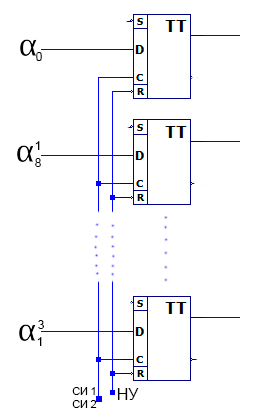
\includegraphics[width=0.4\linewidth]{images/reg}
	\caption{Логическая схема регистров}
	\label{fig:reg}
\end{figure}

\subsection{Разработка регистра признаков результата}

Регистр признаков хранит информацию о результате работы устройства.
Регистр состоит из 4 триггеров.

Первый даёт единицу, если результат положительный, второй -- если отрицательный, третий -- если равен нулю, четвёртый -- если произошло переполнение (при этом первые 3 триггера блокируются).

\begin{figure}[H]
	\centering
	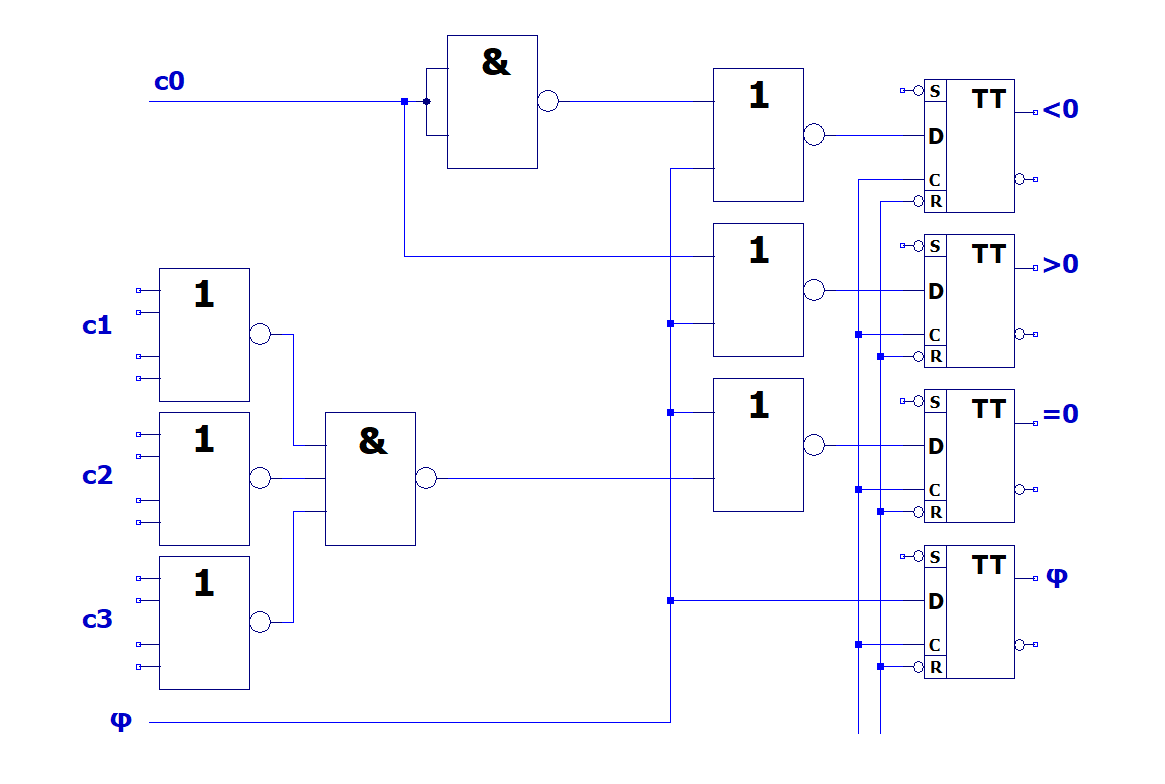
\includegraphics[width=\linewidth]{schemas/prop}
	\caption{Логическая схема регистра признаков}
	\label{fig:prop}
\end{figure}
\subsection{Расчёт временных параметров устройства управления}

Определим временные промежутки (Т1, Т2, Т3) между СИ.

Т1 характеризуется длительностью работы трехразрядного десятичного сумматора.
Для определения необходимо определить задержки сигналов по каждой схеме, которая входит составной частью в общую схему.

В одноразрядном двоичном сумматоре задержка переноса $2ns$, задержка полного вычисления -- $5ns$.

Для одноразрядного десятичного сумматора необходимо найти самую длинную цепь. До корректора самая длинная цепь состоит из трёх переносов и суммы, итого до корректора $11ns$ ($3 * 2ns + 5ns$).
Корректор затрачивает $2ns$ на перенос и $3ns$ на обработку коррекции. 
% Итого, после корректора сумма уже $15ns$.
Далее самая длинная цепочка проходит через 2 переноса в следующий разряд и производится подсчёт суммы -- $2ns * 2 + 5ns = 9ns$.
В сумме одноразрядый десятичный сумматор занимает $11ns + 2ns = 13ns$ на вычисление переноса в следующий разряд и $11ns +3ns + 9ns = 23 ns$ на вычисление значения.

Задержка в преобразователе равна $3ns$.

Схема, фиксирующая переполнение разрядной сетки требует  $3ns$.

В 3-разрядном десятичном сумматоре самой длиной цепью будет следующая цепь:
\begin{enumerate}
	\item Преобразование -- $3ns$
	\item DC3 перенос в следующий разряд -- $13ns$
	\item DC2 перенос в следующий разряд -- $13ns$
	\item DC1 перенос двоичный сумматор -- $13ns$
	\item Двоичный сумматор -- $2ns$
	\item Одноразрядный десятичный сумматор DC3 -- $23ns$
	\item Преобразование -- $3ns$
\end{enumerate}

Результат двоичного сумматора и детектора переполнения успеют подсчитаться за время обработки в сумматоре DC3.

Итого, $3ns + 13ns * 3 + 2ns + 23ns + 3ns = 70ns$

Так как $T_1$ должно быть кратно 4 (длительность  импульса $2ns$ и промежуток $2ns$), то $T_1 = 72ns$.

$T_2$ определяется задержкой во входных цепях регистра признаков, комбинационная схема на входе триггера имеет задержку не превосходящую $4ns$, значит $T_2 = 4ns$.

Величина $T_3$ также равна $4ns$, так как сигнал останова СИ4 идёт непосредственно за сигналом СИ3.

Имея временные интервалы между выходными сигналами в распределителе сигналов, можно приступить к проектированию данного устройства.
Распределитель сигналов является генератором следующих четырёхразрядных двоичных чисел:

$0001,0000 - 17$ раз$, 0010, 0100, 1000$


\subsection{Разработка схемы для получения управляющих сигналов и схемы пуска выполнения операции сложения}

Имея комбинацию выходных сигналов, составим таблицу истинности для генератора сигналов.



\begin{landscape}
	\begin{table}[H]
		\begin{center}
			\caption{\label{tab:rasp} Таблица истинности для генератора сигналов}
			
\begin{tabular}{|c|c|c|c|c?c|c|c|c|c?c|c|c|c|c?c|c|c|c|c?c|c|c|c|}
	\hline
	\multicolumn{5}{|c|}{Такт $n$}        & \multicolumn{5}{c|}{Такт $n+1$}       & \multicolumn{5}{c|}{Значения функций}                                                                  & \multicolumn{5}{c|}{Сигнал на триггер} & \multicolumn{4}{c|}{Сихнхроимпульсы} \\ \hline
	$Q^5$ & $Q^4$ & $Q^3$ & $Q^2$ & $Q^1$ & $Q^5$ & $Q^4$ & $Q^3$ & $Q^2$ & $Q^1$ & $F_5$              & $F_4$              & $F_3$              & $F_2$              & $F_1$              & $D_5$  & $D_4$ & $D_3$ & $D_2$ & $D_1$ & СИ4     & СИ3     & СИ2     & СИ1    \\ \hline
	0     & 0     & 0     & 0     & 0     & 0     & 0     & 0     & 0     & 1     & 0                  & 0                  & 0                  & 0                  & $\bigtriangleup$   & 0      & 0     & 0     & 0     & 1     & 0       & 0       & 0       & 1      \\ \hline
	0     & 0     & 0     & 0     & 1     & 0     & 0     & 0     & 1     & 0     & 0                  & 0                  & 0                  & $\bigtriangleup$   & $\bigtriangledown$ & 0      & 0     & 0     & 1     & 0     & 0       & 0       & 0       & 0      \\ \hline
	0     & 0     & 0     & 1     & 0     & 0     & 0     & 0     & 1     & 1     & 0                  & 0                  & 0                  & 1                  & $\bigtriangleup$   & 0      & 0     & 0     & 1     & 1     & 0       & 0       & 0       & 0      \\ \hline
	0     & 0     & 0     & 1     & 1     & 0     & 0     & 1     & 0     & 0     & 0                  & 0                  & $\bigtriangleup$   & $\bigtriangledown$ & $\bigtriangledown$ & 0      & 0     & 1     & 0     & 0     & 0       & 0       & 0       & 0      \\ \hline
	0     & 0     & 1     & 0     & 0     & 0     & 0     & 1     & 0     & 1     & 0                  & 0                  & 1                  & 0                  & $\bigtriangleup$   & 0      & 0     & 1     & 0     & 1     & 0       & 0       & 0       & 0      \\ \hline
	0     & 0     & 1     & 0     & 1     & 0     & 0     & 1     & 1     & 0     & 0                  & 0                  & 1                  & $\bigtriangleup$   & $\bigtriangledown$ & 0      & 0     & 1     & 1     & 0     & 0       & 0       & 0       & 0      \\ \hline
	0     & 0     & 1     & 1     & 0     & 0     & 0     & 1     & 1     & 1     & 0                  & 0                  & 1                  & 1                  & $\bigtriangleup$   & 0      & 0     & 1     & 1     & 1     & 0       & 0       & 0       & 0      \\ \hline
	0     & 0     & 1     & 1     & 1     & 0     & 1     & 0     & 0     & 0     & 0                  & $\bigtriangleup$   & $\bigtriangledown$ & $\bigtriangledown$ & $\bigtriangledown$ & 0      & 1     & 0     & 0     & 0     & 0       & 0       & 0       & 0      \\ \hline
	0     & 1     & 0     & 0     & 0     & 0     & 1     & 0     & 0     & 1     & 0                  & 1                  & 0                  & 0                  & $\bigtriangleup$   & 0      & 1     & 0     & 0     & 1     & 0       & 0       & 0       & 0      \\ \hline
	0     & 1     & 0     & 0     & 1     & 0     & 1     & 0     & 1     & 0     & 0                  & 1                  & 0                  & $\bigtriangleup$   & $\bigtriangledown$ & 0      & 1     & 0     & 1     & 0     & 0       & 0       & 0       & 0      \\ \hline
	0     & 1     & 0     & 1     & 0     & 0     & 1     & 0     & 1     & 1     & 0                  & 1                  & 0                  & 1                  & $\bigtriangleup$   & 0      & 1     & 0     & 1     & 1     & 0       & 0       & 0       & 0      \\ \hline
	0     & 1     & 0     & 1     & 1     & 0     & 1     & 1     & 0     & 0     & 0                  & 1                  & $\bigtriangleup$   & $\bigtriangledown$ & $\bigtriangledown$ & 0      & 1     & 1     & 0     & 0     & 0       & 0       & 0       & 0      \\ \hline
	0     & 1     & 1     & 0     & 0     & 0     & 1     & 1     & 0     & 1     & 0                  & 1                  & 1                  & 0                  & $\bigtriangleup$   & 0      & 1     & 1     & 0     & 1     & 0       & 0       & 0       & 0      \\ \hline
	0     & 1     & 1     & 0     & 1     & 0     & 1     & 1     & 1     & 0     & 0                  & 1                  & 1                  & $\bigtriangleup$   & $\bigtriangledown$ & 0      & 1     & 1     & 1     & 0     & 0       & 0       & 0       & 0      \\ \hline
	0     & 1     & 1     & 1     & 0     & 0     & 1     & 1     & 1     & 1     & 0                  & 1                  & 1                  & 1                  & $\bigtriangleup$   & 0      & 1     & 1     & 1     & 1     & 0       & 0       & 0       & 0      \\ \hline
	0     & 1     & 1     & 1     & 1     & 1     & 0     & 0     & 0     & 1     & $\bigtriangleup$   & $\bigtriangledown$ & $\bigtriangledown$ & $\bigtriangledown$ & $\bigtriangledown$ & 1      & 0     & 0     & 0     & 0     & 0       & 0       & 0       & 0      \\ \hline
	1     & 0     & 0     & 0     & 1     & 1     & 0     & 0     & 0     & 1     & 1                  & 0                  & 0                  & 0                  & $\bigtriangleup$   & 1      & 0     & 0     & 0     & 1     & 0       & 0       & 0       & 0      \\ \hline
	1     & 0     & 0     & 0     & 1     & 1     & 0     & 0     & 1     & 1     & 1                  & 0                  & 0                  & $\bigtriangleup$   & $\bigtriangledown$ & 1      & 0     & 0     & 1     & 0     & 0       & 0       & 0       & 0      \\ \hline
	1     & 0     & 0     & 1     & 1     & 1     & 0     & 0     & 1     & 1     & 1                  & 0                  & 0                  & 1                  & $\bigtriangleup$   & 1      & 0     & 0     & 1     & 1     & 0       & 0       & 1       & 0      \\ \hline
	1     & 0     & 0     & 1     & 1     & 1     & 0     & 1     & 0     & 0     & 1                  & 0                  & $\bigtriangleup$   & $\bigtriangledown$ & $\bigtriangledown$ & 1      & 0     & 1     & 0     & 0     & 0       & 1       & 0       & 0      \\ \hline
	1     & 0     & 1     & 0     & 0     & 0     & 0     & 0     & 0     & 0     & $\bigtriangledown$ & 0                  & $\bigtriangledown$ & 0                  & 0                  & 0      & 0     & 0     & 0     & 0     & 1       & 0       & 0       & 0      \\ \hline
\end{tabular}
			
		\end{center}
	\end{table}
\end{landscape}


\section{Общая структура схемы многоразрядного десятичного сумматора комбинационного типа с устройством управления}

\section{Выводы по работе}

\end{document}